\documentclass[10pt]{reportMaster}
\usepackage[utf8]{inputenc}
\usepackage{graphicx} % To handle images
\usepackage[font=small,labelfont=bf]{caption}
\usepackage[font=footnotesize,labelfont=bf]{subcaption}
\usepackage{algorithmic} % For algorithm and pseudocode
\usepackage{amsmath} 
\usepackage{mathtools}
\usepackage{verbatim} % For multi-line commenting
\usepackage{url}
\usepackage{todonotes}

\title{{Predicting Tumor Hypoxia Map from FDG-PET/CT using GANs}}
\author{C. Rao}
\id{DKE-21-24}
\nameMastersProgramme{Artificial Intelligence}
\committee{Dr. A. Briassouli \\ Dr. E. Hortal Quesada}
\date{March 16, 2021} % TODO: Change to appropriate date

\begin{document}

\maketitle

% Abstract
\begin{abstract}
    Add abstract ...  
\end{abstract}

% Table of contents
\tableofcontents

% Chapters
\chapter{Introduction}
\label{Introduction}

\section{Problem Statement}
Tumor hypoxia is a condition wherein certain regions within the tumor volume are deprived of oxygen, and is caused when the tumor's blood supply system cannot keep up with the proliferation rate of its cells \cite{hockel2001tumor}. Hypoxic cells develop certain alterations in their functioning mechanisms that make them resistant to conventional modes of cancer treatment, including radiotherapy and chemotherapy, and increase metastatic spread \cite{muz2015role}, thereby resulting in poor prognosis \cite{vaupel2007hypoxia}. In radiotherapy, it would be of great value to detect these hypoxic sub-volumes during treatment planning so that the radiation dose can be adjusted accordingly to be more effective, for example, by selectively delivering higher dose to the hypoxic regions, a technique known as radiotherapy boosting. Among various non-invasive methods investigated for hypoxia detection, Positron Emission Tomography (PET) based hypoxia imaging has been the most preferred one \cite{fleming2015imaging}. PET is a molecular imaging technique that involves administration of a specific radioactive pharmaceutical contrast agent, known as radiotracer, to the patient, followed by tracking it via scanning to provide information about the status of a particular biochemical process. Hypoxia PET imaging provides, essentially, an oxygen concentration heatmap which can be overlaid on a Computer Tomography (CT) scan to provide contrast around the anatomical regions that are hypoxic. A newly developed hypoxia tracer, denoted as [$^{18}$F]HX4, has been shown to be highly effective and stable in detecting regions of tumor hypoxia \cite{sanduleanu2020hypoxia}, and the PET image acquired using this tracer is denoted as HX4-PET. HX4-PET imaging technique, however, is not widely available, is expensive and has only been used in research and clinical trials so far. 

Generative adversarial networks (GANs) have recently become a subject of investigation as a general solution to image-to-image translation problems. The Pix2pix and CycleGAN frameworks \cite{isola2017image, zhu2017unpaired} are among the early systems developed in this direction targeting paired and unpaired variants of the problem, respectively. While paired translation tasks supply spatially aligned pairs of input and target images in the training data to directly learn an input-target mapping, unpaired translation tasks do not provide paired data usually because it is either impossible, unrealistically difficult or unacceptably risky to obtain such data. In the space of medical imaging, GAN-based techniques have been widely explored for translating images of one modality into another \cite{yi2019generative}. However, since medical images are quantitative in nature that represent some underlying physical or biochemical properties of human body, and since these images are used for clinical decision making, the GAN-generated synthetic images must be representative of the patient's condition and must conform to high quality standards. Evaluation of synthetic medical images is a difficult problem and is, in many cases, application-specific. 

It would be of great benefit to patients and to the care provider if entire HX4-PET images could be synthesized from more readily available imaging modalities. FDG-PET, which indicates metabolism levels, and CT images have been shown to contain features capable of reliably predicting hypoxic regions in the tumor \cite{even2017predicting, sanduleanu2020non}, and to have the potential of circumventing the use of HX4-PET imaging. The problems tackled by this thesis project are two-fold -- (1) Synthesis of full HX4-PET images from FDG-PET and CT scans of the patients using GANs, and (2) Evaluation of different aspects of the synthetic HX4-PET images using general image quality metrics and via application-specific image analysis.



\section{Significance of the Thesis}
This work formulates the hypoxia prediction problem as an image-to-image translation task where entire 3D HX4-PET images are to be synthesized from FDG-PET and CT. We investigate both paired and unpaired GAN approaches, specifically Pix2Pix and CycleGAN, as potential solutions to this problem. CycleGAN system utilizes cycle-consistency to learn an image translation model in the absence of paired training data by simultaneously learning an input-target mapping as well as its inverse. However, since the input in our use-case is multimodal, applying CycleGAN naively to this problem may not be optimal. CycleGAN assumes the existence of a bijective function between the input and the target domains, which is violated here as it is practically impossible to precisely reconstruct both FDG-PET and CT back from a single HX4-PET. Therefore, in order to sidestep this issue, a design improvement in the CycleGAN training is proposed for this specific use-case. To our best knowledge, ours is the first work that has attempted GAN-based cross-modality medical image translation involving more than two imaging modalities.

To address the problem of evaluating synthetic HX4-PET images, we use six different metrics that measure different properties of an image, including voxel-wise difference, fidelity of the perceived structure and global intensity statistics. Since each metric has its unique strengths and drawbacks, our aim is to use metrics of different types to complement each other and reach a consensus on the models' assessment. Based on these metrics, we empirically show that the modified CycleGAN achieved remarkable improvement over the default CycleGAN, and we simultaneously validate the assessment of these metrics by performing a systematic visual inspection of the 3D synthetic images. Additionally, we investigate the applicability of these image quality metrics in tracking the stability and convergence of the CycleGAN models during training.

Finally, we perform a clinically relevant analysis of the synthetic HX4-PET images to determine their clinical value. Application-specific downstream tasks are identified from hypoxia imaging literature and applied to quantify hypoxia locally within the tumors. This is of great importance and of more interest to clinicians as a benchmark to gauge the potential of the models as an alternative solution to HX4-PET imaging to be integrated into radiotherapy practice in future. Although our quantitative results on tumor hypoxia quantification indicate no significant performance difference among the different methods, our qualitative analysis highlights the drawbacks of paired GAN approaches and suggests that unpaired methods might be more suitable for the task, given sufficient data.



\section{Research Questions}
The research questions posed initially at the time of drafting the thesis plan were slightly updated, without changing their overall theme, later when the work on the project actually began. The primary reason is that the exact specifications of the project were not provided earlier, rather only a vague formulation of the problem was given -- synthesis of Contrast-Enhanced Computed Tomography (CECT) images from CT using GANs. ``Contrast-enhanced" CT is an umbrella term that includes a variety of techniques used to selectively provide contrast enhancement to certain regions in a CT scan, ranging from using iodine-based contrast agents that improve visibility of organs like liver and pancreas by raising the radiodensity of blood to acquiring PET scans that utilize radiotracers to highlight sites of certain physiological processes like metabolism and hypoxia. Therefore, one of the main changes in the research questions was replacing the term ``CECT" with ``HX4-PET". Reasons for other question-specific changes are provided further in \ref{updated_research_questions}.


\subsection{Original}
\begin{enumerate}
    \item What measures need to be considered during evaluation to more accurately quantify the similarity of synthetic CECT images with clinically acquired ones in an unpaired image-to-image translation scenario?
    \item How reliable are deep-learning based downstream analysis approaches, such as image classification or segmentation, for evaluating synthetic CECT images?
    \item How can such application-specific validation methods be applied to assess the stability of CycleGAN training for this task and detect issues like mode collapse?
\end{enumerate}


\subsection{Updated}
\label{updated_research_questions}

\begin{enumerate}
    \item What measures need to be considered during evaluation to accurately quantify the similarity of synthetic HX4-PET images with the clinically acquired scans?
    \item How can application-specific downstream image analysis aid in evaluating the utility of synthetic HX4-PET images for tumor hypoxia measurement?
    \item To what extent can image quality metrics provide information on convergence of the GAN models during training?
\end{enumerate}

All question-specific changes were made to make the questions more sensible and meaningful. In Question 1, the phrase ``in an unpaired image-to-image translation scenario" was removed because in the medical image dataset used in this project, the ground-truth is available, especially for the validation images, and the evaluation can be performed by merely comparing the predictions with the ground-truth, whether or not the training was performed in an unpaired manner. In Question 2, the phrase ``deep-learning based downstream analysis" was replaced with ``application-specific downstream analysis" because simpler thresholding based hypoxia classification and segmentation techniques are sufficient for image analysis. Since PET images are quantitative in nature, standardized intensity thresholds are already established for the downstream tasks and have been used in previous HX4-PET related clinical studies \cite{zegers2013hypoxia, even2017predicting, sanduleanu2020hypoxia}. Using deep-learning to perform these downstream tasks would not only be unnecessary and less reproducible, but also infeasible due to the small size of the dataset. This question now focuses on the tumor region and the value that synthetic HX4-PET image can provide in a clinical scenario in predicting hypoxia patterns within this region, instead of focusing on the overall quality and perfectness of the full image. This is reasonable because the tumor region is already delineated prior to HX4-PET acquisition. In Question 3, the phrase ``application-specific validation methods" was replaced with ``image quality metrics" because otherwise, the question would be invalid. This reason being that ``application-specific methods" implies hypoxia analysis methods (which is addressed in Question 2), which are not suitable for measuring the overall quality of the full synthetic HX4-PET images since the tumor size is much smaller than the size of the full image. To decide whether or not a GAN model is converging during training, one needs to check the overall quality of the its generated samples. Therefore, this question can now be viewed as an extension of Question 1 and as being complementary to Question 2. 
\chapter{Related Work}
\label{Related_Work}



%%%%%%%%%%%%%%%%%%%%%%%%%%%%%%%%%%%%%%%%%%%%%%%%%%%%%%%%%%%%%%%%%%%%%%%%%%%%%%%%%%%%%%%%%%%%%%%%%%%%%%%%%%%%%%%%%%%%%%%%%%%%%%%%%%%%%%%%%%%%%%%
\section{Predicting Hypoxia from FDG-PET and CT}
\label{Related_Work-hypoxia_prediction}
In a hypoxia PET image, the tumor is the sole object of interest whose exact location and shape is usually known before the hypoxia image acquisition. Zegers et al. \cite{zegers2014vivo} show the presence of significant correlation among tumor-level parameters -- tumor size, overall tumor metabolism (indicated by FDG-PET uptake) and overall tumor hypoxia (indicated by HX4-PET uptake). They additionally perform sub-volume level (i.e. voxel-wise) analysis between FDG-PET and HX4-PET to evaluate the spatial similarity of both tracers' uptake patterns within the tumor, and observe a reasonable correlation between them. However, they also note that this correlation is not significant likely due to the involvement of genetic properties of the tumor, and conclude that HX4-PET imaging does indeed provide information complementary to FDG-PET. Even et al. \cite{even2017predicting} investigate the possibility of predicting hypoxia patterns in the tumor using other indirect markers of hypoxia including anatomy (CT), metabolism (FDG-PET), and blood perfusion parameters (tumor blood flow and blood volume maps obtained from Dynamic CT). They argue that a voxel-wise regression between the inputs and the HX4-PET ground truth would be negatively affected by registration-related imperfections, and instead use a supervoxel based approach for robustness. They train random-forest-based regression models on simple features -- median, standard deviation and entropy -- derived from the supervoxels in each input image modality to infer the level of hypoxia in the corresponding supervoxel regions. The models were shown to reliably predict the spatial distribution of tumor hypoxia, and the features from CT and FDG-PET were found to be the most informative. Sanduleanu et al. \cite{sanduleanu2020non} conduct a large-scale radiomic study using data from six different medical centers. Radiomic features comprise a large set of standardized quantitative features extracted from medical images developed with the aim of supporting high-throughput automated image analysis in radiation oncology \cite{aerts2014decoding}. The authors hypothesize that the combined radiomic features derived from both CT and FDG-PET modalities can predict tumor hypoxia status more effectively compared to either of these modalities alone, and build and validate multiple random-forest-based tumor classification models. They conclude with the finding that the radiomic models using both modalities did indeed classify the tumors as hypoxic or non-hypoxic with high accuracy.

In this work, we utilize CT and FDG-PET information and aim at predicting hypoxia patterns in the entire body region covered by the input images, instead of focusing on just the tumor locality. In order to synthesize full HX4-PET images accurately, the HX4 tracer uptake in the human body must be effectively modeled as a function of CT-derived anatomical features and FDG tracer uptake. Then, inferring the HX4 uptake within the tumor becomes a special case of inferring it at any given region in the body, and this special case is characterized by the presence of abnormal structures in CT and an immense amount of activity in FDG-PET.



%%%%%%%%%%%%%%%%%%%%%%%%%%%%%%%%%%%%%%%%%%%%%%%%%%%%%%%%%%%%%%%%%%%%%%%%%%%%%%%%%%%%%%%%%%%%%%%%%%%%%%%%%%%%%%%%%%%%%%%%%%%%%%%%%%%%%%%%%%%%%%%
\section{Image-to-Image Translation GANs}
Generative adversarial networks (GANs) \cite{goodfellow2014generative} are a class of deep generative models comprised of two networks -- the generator and the discriminator -- that are jointly trained in a competitive setting. The generator's task is to synthesize samples (often images) that are indistinguishable from samples from the true data distribution, whereas the task of the discriminator is to accurately distinguish between real and synthetic samples. Over the training period, the generator learns to produce increasingly realistic samples in response to the discriminator's feedback, which itself also improves. The model eventually converges to an equilibrium state where the generator ideally models the real data distribution, and as a result, the best the discriminator can do is random guessing. While the user has no control over the semantics of the images generated by the GAN model, the development of Conditional GAN (cGAN) \cite{mirza2014conditional} has allowed using simple semantic information, such as class labels, to train a conditional generative model. During inference, this enables the user to query the generator to synthesize images belonging to a given class. 

Based on cGAN, Isola et al. \cite{isola2017image} introduce the Pix2Pix system as a general-purpose framework for solving image-to-image translation problems. Any computer vision or graphics task that takes as input an image and expects another image as its output having the same size and containing the same semantic information can be formulated as image-to-image translation. For example, semantic segmentation of photographs, synthesis of photographs from semantic label map or edge map, and colorization of monochrome photos. In such problems, the input and the output images are viewed as different renderings of the same underlying scene. The Pix2Pix generator, conditioned on the entire input image, produces an output image that is directly compared to the ground truth via a pixel-wise L1 loss. Additionally, as a consequence of the adversarial training, the Pix2Pix discriminator model serves as a ``structured" loss function that is learned from the data itself. This essentially rules out the need to handcraft custom loss functions for each image translation task. Pix2Pix, however, requires pixel-wise aligned input-target image pairs, i.e. \textit{paired} data, for training. A classic example task where paired data doesn't exist is horse-to-zebra translation \cite{zhu2017unpaired}. Based on ideas similar to Pix2Pix, Zhu et al. present the CycleGAN system \cite{zhu2017unpaired} for learning an image translation model from unpaired data. CycleGAN consists of four deep neural networks, which compose two generator-discriminator pairs. Given two sets of images, each containing images of one \textit{domain}, the CycleGAN model learns a forward mapping between the input and the target domains as well as its inverse. This pair of mappings is used to implement a cycle-consistency mechanism to encourage the preservation of high-level structure (i.e. the ``content") across an input image and its translated counterpart in the target domain. Since there is no direct way to ensure content preservation between input and output images due to the absence of paired data, this strategy serves as an indirect means to achieve this.

The Pix2Pix and CycleGAN systems have been widely applied in medical imaging research to various cross-modality image translation use cases \cite{yi2019generative} with slight custom modifications in network architecture and loss functions, although we limit our discussion to works that focus on synthesizing contrast maps from CT images. Chandrashekar et al. \cite{chandrashekar2020deep} show that sufficient contrast exists between blood and soft tissue to differentiate them in CT angiograms acquired without a contrast agent, and train a 2D CycleGAN model to selectively enhance the existing contrast and accurately simulate iodine-based contrast effect in the CT images. Haubold et al. \cite{haubold2021contrast} instead investigate into reducing the amount of required iodine-based contrast agent dose from full dose to as low as 50\%, and apply a 2D Pix2Pix-based post-processing step to provide the remaining contrast to the CT. Motivated by the drawback of multimodal FDG-PET/CT-based lesion detection systems requiring FDG-PET acquisition, Ben-Cohen et al. \cite{bencohen2018crossmodality} investigate synthesizing FDG-PET images from just CT scans. The authors use a two-step approach combining a fully convolutional regression network with a Pix2Pix GAN. They argue that CT-derived synthetic FDG-PET can potentially substitute a clinically acquired FDG-PET scan for improving tumor visibility, although they do not provide any physiological basis for image translation problem. Bi et al. \cite{bi2017synthesis}, as opposed to other studies which focus on the direct clinical application of synthetic images, aim at synthesizing realistic FDG-PET samples for providing data augmentation to train auxiliary deep-learning-based systems, for example, malignancy detection models. In order to preserve the position and shape of the tumor across translation, they utilize explicitly the tumor annotation together with the CT image in a two-channel Pix2Pix model to generate the corresponding FDG-PET. 

Based on our literature survey, we found no prior work that investigated cross-modality translation for synthesizing hypoxia PET from other modalities. We explore both the paired and unpaired image translation approaches, using Pix2Pix and CycleGAN systems, respectively, since they are among the most straightforward and widely applied image translation methods.



%%%%%%%%%%%%%%%%%%%%%%%%%%%%%%%%%%%%%%%%%%%%%%%%%%%%%%%%%%%%%%%%%%%%%%%%%%%%%%%%%%%%%%%%%%%%%%%%%%%%%%%%%%%%%%%%%%%%%%%%%%%%%%%%%%%%%%%%%%%%%%%
\section{Evaluation of Synthetic Medical Images}

Evaluation of GAN-translated synthetic images is a difficult problem even when the ground truth reference images are available. In quantitative medical images, pixel-wise differences such as mean-squared error (MSE) and peak signal-to-noise ratio (PSNR) can be useful in only partially assessing image quality since they do not account for the image statistics and local structure. Perceptual metrics like structural similarity index (SSIM) have, therefore, been widely applied to assess the synthetic images based on the similarity of their perceived local structure with that of the ground truth \cite{yi2019generative}. Image registration literature provides entropy-based metrics for image matching, such as normalized mutual information (NMI) \cite{studholme1999overlap}, that can measure structural alignment even across different image modalities. Mutual information has been applied as an image quality metric in works concerning translation across Magnetic Resonance (MR) image sequences \cite{yang2018mri, welander2018generative}. 

In many cases, the end goal of the synthetic images is to potentially substitute the clinically acquired scans, and therefore, image evaluation must be application-specific and clinically relevant. It is, therefore, common to perform downstream tasks using synthetic images to measure their clinical value. Haubold et al. \cite{haubold2021contrast} include in their evaluation a manual ``pathological consistency" testing procedure where synthetic image slices are compared to their corresponding ground truth slices by trained radiologists to check whether the synthetic image preserves the patient's existing pathology and doesn't insert pathology that is non-existent in the ground truth. Ben-Cohen et al. \cite{bencohen2018crossmodality} evaluate their synthetic FDG-PET images by using them, in combination with CT, to detect lesions in the image and measuring the detection performance.  

We perform an evaluation on our synthetic HX4-PET images via both general image quality metrics and application-specific downstream image analysis. Because each image quality metric has its own strengths and weaknesses, we use a multitude of them to effectively quantify the fidelity of the synthetic images. Additionally, a systematic visual inspection is performed to identify common failure modes of the image translation GANs used. As downstream tasks, we perform binary classification of the tumors as hypoxic or non-hypoxic and segmentation of the 3D hypoxic regions within the tumor. HX4-PET images are quantitative in nature and have established procedures for hypoxia quantification \cite{zegers2013hypoxia}. The hypoxia quantification tasks are, therefore, performed using simple thresholding-based methods with standard threshold values derived from the relevant clinical literature \cite{zegers2013hypoxia, even2017predicting}.
\chapter{Methodology}
\label{Methodology}


\section{Software and Hardware}
\todo{write this}

For certain specialized tasks, such as PET SUV calculation and RTstruct conversion, parts of source code from a public repository \footnote{\url{https://github.com/voreille/hecktor}} were used to ensure the correctness of the implementation. This code repository contains utility code created as part of the HECKTOR PET/CT segmentation challenge \cite{andrearczyk2020overview} by its authors.

% FDG SUV calculation
For the sake of correctness of the implementation of this formula, utility code from the HECKTOR repository was used to perform this conversion \footnote{BQML to SUV conversion code: \url{https://bit.ly/33IG4Jg}}.




%%%%%%%%%%%%%%%%%%%%%%%%%%%%%%%%%%%%%%%%%%%%%%%%%%%%%%%%%%%%%%%%%%%%%%%%%%%%%%%%%%%%%%%%%%%%%%%%%%%%%%%%%%%%%%%%%%%%%%%%%%%%%%%%%%%%%%%%%%%%%%%
\section{Data}
% Image modalities involved and their properties
% The Maastro Lung HX4 dataset
% Data processing
The medical imaging dataset used in this project, hereafter referred to as \textit{Maastro Lung HX4 dataset}, is a combination of two different datasets originally acquired for two clinical trials at Maastro, and was also previously used by Even et al. \cite{even2017predicting} in their hypoxia prediction study. It includes 3D scans of 34 Non-Small Cell Lung Cancer (NSCLC) patients in total, of which 15 belong to the \textit{PET-Boost} trial (registration number NCT01024829) \cite{van2012pet} and 19 to the \textit{Nitroglycerin} trial (registration number NCT01210378) \cite{even2017predicting}. The request for the usage of this data in this project was approved by the institutional review board (IRB).


% -------------------------
\subsection{Original Scans}
\label{Original_Scans}
In the original dataset, each individual scan was stored as a separate DICOM series \footnote{DICOM is an international standard for storing and managing medical images: \url{https://www.dicomstandard.org/}} which contained the image intensity data, the spatial information of the image and the image acquisition details. The first set of images for each patient included the Planning FDG-PET/CT images, where the CT component was the radiotherapy treatment planning CT (pCT). Both images were acquired using a single hybrid scanner and were, hence, registered with each other by default. The 3D field-of-view (FOV) of both images included the patient's chest, although the FOV of pCT was different than that of FDG-PET. Spatial resolution of all FDG-PET images was 4$\times$4$\times$3 mm$^3$ and that of the pCT was 0.97$\times$0.97$\times$3 mm$^3$, specified in the \textit{x}$\times$\textit{y}$\times$\textit{z} format. Additionally, annotations of certain structures relevant to the treatment planning process, for example, the primary tumor, nearby organs-at-risk, and the patient's body, were provided for each patient in the DICOM \textit{RTstruct} format \footnote{Radiotherapy structure set (RTstruct) is the DICOM-specified format for storing radiotherapy-related annotations: \url{https://dicom.innolitics.com/ciods/rt-structure-set}}. These structures were delineated by a radiation oncologist on the Planning CT (pCT). Figure \ref{fig:original_fdgpet_pct} shows a visualization of FDG-PET and pCT images of a sample patient.

\begin{figure}[h!]
    \centering
    \includegraphics[width=\linewidth]{figures/Data/original/N010-FDG_PET_pCT.png}
    \caption{Single coronal (\textit{x}-\textit{z} plane) slice of FDG-PET and pCT images. White bounding boxes show their respective FOVs. Radiotherapy structure annotations were provided for pCT of which three are shown here -- the patient's body (green), the lungs (dark blue) and the primary tumor (red). The FDG tracer has high specificity to metabolism, resulting in high contrast near the tumor.}
    \label{fig:original_fdgpet_pct}
\end{figure}

The second set of images included the HX4-PET and the accompanying low-dose CT (ldCT). For each patient, these were acquired on a different day than their corresponding FDG-PET/pCT scans. Both images were simultaneously acquired (thus, aligned with each other by default), and they cover approximately the same FOV of the patient's chest. However, the FOV covered by HX4-PET/ldCT couple was more focused on the tumor and was smaller in the axial direction compared to the FDG-PET/pCT couple. The HX4-PET images had a resolution of 4$\times$4$\times$4 mm$^3$ and the resolution of ldCT was 1.17$\times$1.17$\times$4 mm$^3$. Figure \ref{fig:original_hx4pet_ldct} shows a visualization of sample HX4-PET and ldCT images.

\begin{figure}[h!]
    \centering
    \includegraphics[width=\linewidth]{figures/Data/original/N010-HX4_PET_ldCT.png}
    \caption{Single coronal slice of HX4-PET and ldCT images. Both had similar FOVs. No annotations were provided for the ldCT.}
    \label{fig:original_hx4pet_ldct}
\end{figure}

Both the CT images -- pCT and ldCT -- had their voxel intensity values expressed in terms of the Hounsfield Unit (HU), which is related to the radiodensity of materials. In case of FDG-PET, the units represent levels of radioactivity emitted from the FDG tracer in different parts of the body as measured by the scanner, and were represented in terms of Becquerel per milliliter (Bq/mL, abbreviated as BQML). In HX4-PET, however, intensities were expressed in terms of a different unit called \textit{counts} (abbreviated as CNTS). This unit is specific to the manufacturer, and possibly also to the model, of the PET/CT scanner (Philips Gemini TF64) that was used for HX4-PET acquisition. Before using them for any purpose, FDG-PET and HX4-PET needed their intensity values to be converted to Standardized Uptake Values (SUV) which is the standard unit for PET intensity representation. SUV calculation is discussed in further detail in \ref{data_proc_phase_1}.


% -----------------------------
\subsection{Image Registration}
Note that although each of the two PET/CT couples -- FDG-PET/pCT and HX4-PET/ldCT -- had the PET and CT components aligned with each other by default, both PET/CT couples did not align organ-to-organ with \textit{each other} because they had different \textit{physical} reference frames due to both being acquired in different scanning sessions. Having a version of HX4-PET that is registered to the FDG-PET/pCT was essential to serve as a ground-truth image for evaluating the GANs as well as for paired training of Pix2Pix. Even et al. \cite{even2017predicting} describe a registration procedure for achieving this alignment. They use a two-step approach where the ldCT is first subjected to rigid alignment followed by non-rigid elastic registration over the pCT. The resulting transformation parameters are then applied to the HX4-PET image. Figure \ref{fig:reg_images} shows an example of HX4-PET image before and after registration. 

\begin{figure}[h!]
    \centering
    \includegraphics[width=\linewidth]{figures/Data/reg/N046-HX4_PET_ldCT-unreg_reg.png}
    \caption{Overlaid HX4-PET and ldCT images of a patient before and after registration to pCT, showing axial (top) and sagittal (bottom) slices. pCT is not shown. The scanner table is visible in the ldCT background, and shows the effects of the elastic transformation. Some registration errors are observed here. For example, in the axial slice, the HX4-PET region close to the patient's top surface is overly warped towards the inside resulting in an empty region of zero intensity. Also, in the sagittal slice in (b), some voxels at the bottom are missing the hypoxia signal due to warping.}
    \label{fig:reg_images}
\end{figure}{}

The Maastro Lung HX4 dataset already included the registered HX4-PET and ldCT images, and therefore this registration step wasn't needed to be performed. These images were supplied in the \textit{.mhd/.raw} format. The intensity values of the stored registered HX4-PET were expressed in SUVs, supposedly calculated before the registration process. 

To distinguish the registered HX4-PET from the unregistered one, the two are denoted as \textit{HX4-PET-reg} and \textit{HX4-PET-unreg}, respectively. The term \textit{HX4-PET} is used hereafter to denote the image modality in a general sense and not referring to the registered or unregistered versions of the images from the dataset. It is obvious that FDG-PET and pCT were needed since both would be the inputs to the GANs, and HX4-PET-reg to be the ground-truth given these inputs. And since HX4-PET-reg contained registration imperfections as seen in Figure \ref{fig:reg_images}, the HX4-PET-unreg instead would be used in the unpaired CycleGAN training to sidestep this issue. The \textit{unregistered} ldCT, \textit{ldCT-unreg}, would play a crucial role in the modified CycleGAN system as discussed further in \ref{data_requirements}, and hence was not discarded. However, the \textit{registered} ldCT wouldn't be required anymore beyond this point since its sole purpose was to aid in the registration of HX4-PET, and was thus discarded.


% --------------------------------
\subsection{Data Processing Steps}
\label{Data_Processing}
The Maastro Lung HX4 dataset needed to be prepared and converted into a form that could be used for GAN training. The different processing steps performed on the data are discussed here. The overall data processing can be broken down into two phases, which are elaborated in the following paragraphs. 

\subsubsection{Loading Images and Converting to Appropriate Representation}
The first step was to load the images from different formats into computer memory and convert to a standard programmatic representation. All the original images, except for HX4-PET-reg, were supplied as DICOM series. 

\vspace{4mm}
\noindent
\textit{SUV Calculation:} First, The FDG-PET and HX4-PET-unreg intensity values needed to be converted into the SUV scale. When the intensity units are expressed as BQML, as with all FDG-PET images here, the patient's body weight as well as imaging parameters including the decay time and the total administered dose of the radiotracer are required to calculate the SUV. Equation \ref{BQML_to_SUV} shows the conversion formula. 
\begin{equation}
    SUV = \frac{BQML * 1000 * Weight}{Dose * 2^{-t/\tau}} 
    \label{BQML_to_SUV}
\end{equation}
where $2^{-t/\tau}$ is the decay correction factor at time of acquisition \textit{t}, given the half-life $\tau$ of the radiotracer. The values for the patient's weight, administered dose and decay parameters are stored in the DICOM image series as metadata, which was accessed using the PyDicom library. 

HX4-PET-unreg images, however, were represented in terms of the non-standard CNTS units here, for reasons discussed earlier in \ref{Original_Scans}. CNTS to SUV conversion was performed using the formula implemented in this \footnote{CNTS to SUV conversion code: \url{https://bit.ly/3wbtGgW}} public GitHub repository.

\vspace{4mm}
\noindent
\textit{Conversion of RTstruct Contours to Binary Masks:} RTstruct is the format defined in the DICOM standard for storing radiotherapy-related annotations (known as "radiotherapy structure sets") in the form of contour points. The RTstruct file is stored separately from the scans. Since the process of radiotherapy treatment planning involves creating these contours over the Planning CT (pCT), the physical coordinate system of the pCT scan is the reference frame for the contour points. Of all the different objects annotated in the pCT scan, only the contours for the primary tumor and the patient's body were selected and converted to binary masks. Each of these masks have the same 3D size and resolution as the pCT image. The tumor mask would be needed during evaluation of the hypoxia maps predicted by the models, whereas the body mask would be required during their training to mask away and remove out-of-body objects in scans, for example, the scanner table. The algorithm implemented in this \footnote{RTstruct to binary mask conversion code: \url{https://bit.ly/2RnNI9t}} GitHub repository was used to perform the RTstruct-to-binary-mask conversion.

\begin{figure}[h!]
    \centering
    \includegraphics[width=0.9\linewidth]{figures/Data/data_processing_overview-step_1.png}
    \caption{Overview of the first phase of data processing. Images were loaded from storage into computer memory in a standard programmatic representation.}
    \label{fig:data_proc_overview_1}
\end{figure}

Following this, the FDG-PET, HX4-PET-unreg, pCT and the tumor and body masks were converted to SimpleITK objects in Python. The ldCT-unreg was also loaded using PyDicom and converted to this representation. HX4-PET-reg, stored in \textit{.mhd/.raw} format containing pre-computed SUV values, was directly loaded into a SimpleITK object. Figure \ref{fig:data_proc_overview_1} shows a visual overview of these steps.


\subsubsection{Cropping and Resampling}

\begin{figure}[h!]
    \centering
    \includegraphics[width=\linewidth]{figures/Data/fdgpet_pct_crop1/N010-FDG_PET_pCT-uncropped_crop1.png}
    \caption{Stage 1 cropping of FDG-PET, pCT and the tumor and body masks (not shown here) to a common FOV. Uncropped FDG-PET and pCT are overlaid to show the overlap of their FOVs.}
    \label{fig:fdg_pet_pct_crop1}
\end{figure}

\begin{figure}[h!]
    \centering
    \includegraphics[width=\linewidth]{figures/Data/fdgpet_pct_fx4petreg_crop2/N010-fdgpet_pct_hx4petreg-uncropped_crop2.png}
    \caption{Stage 2 cropping of the input images (FDG-PET and pCT), the masks (tumor and body, not shown here) and the ground truth (HX4-PET-reg) to a common FOV. All FOVs are displayed to show their overlap.}
    \label{fig:fdgpet_pct_hx4petreg_crop2}
\end{figure}

The second data processing phase involved cropping and resampling the loaded images. A standard resampling resolution of 1$\times$1$\times$3 mm$^3$ was chosen. Cropping was performed in a progressive manner as described in the following steps: 

\begin{enumerate}
    \item \textit{Cropping and resampling FDG-PET, pCT and masks:} As shown earlier in \ref{Original_Scans}, the FOVs of FDG-PET and pCT are different. Both images needed to be cropped such that both would contain the same FOV of the patient. This can be solved by finding the 3D volumetric intersection of both their FOVs and cropping to this new volume size. The resampling step was performed immediately following this. The tumor and body masks share the same FOV with pCT, and hence, were cropped the same way as pCT was. This is the Stage 1 cropping of FDG-PET, pCT and the masks. Figure \ref{fig:fdg_pet_pct_crop1} illustrates this step.

    \item \textit{Cropping and resampling HX4-PET and ldCT:} The same process of cropping to common FOV followed by resampling was performed on HX4-PET-unreg and ldCT-unreg images. This is the Stage 1 cropping of HX4-PET-unreg and ldCT-unreg.

    \item \textit{Resampling HX4-PET-reg:} The HX4-PET-reg image was then just resampled to the standard resolution.

    \item \textit{Cropping the input images, the masks and the ground-truth image to common FOV:} Furthermore, the two input images (FDG-PET and pCT), the two masks and the ground-truth image (HX4-PET-reg) were cropped to the common FOV among them. The reason being that although HX4-PET-reg is organ-to-organ aligned with the input images and all of them have a common physical reference frame (due to registration), its FOV is different. This is the Stage 2 cropping. Figure \ref{fig:fdgpet_pct_hx4petreg_crop2} shows a visualization of this step.
\end{enumerate}

\begin{figure}[h!]
    \centering
    \includegraphics[width=0.8\linewidth]{figures/Data/data_processing_overview-step_2.png}
    \caption{Overview of the second phase of data processing.}
    \label{fig:data_proc_overview_2}
\end{figure}

Finally, all the processed images were saved as \textit{.nrrd} files. The NRRD format allows storage of N-dimensional raster images along with their spatial information, including voxel spacing (resolution) and physical coordinates of the origin, as a single file. Figure \ref{fig:data_proc_overview_2} shows an overview of the entire second phase of data processing discussed thus far. The dataset was then split into a training set and a validation set. The training set was comprised of data from the PET-Boost clinical trial (15 patients), and the validation set consisted of the data from the Nitroglycerin trial (19 patients). 



%%%%%%%%%%%%%%%%%%%%%%%%%%%%%%%%%%%%%%%%%%%%%%%%%%%%%%%%%%%%%%%%%%%%%%%%%%%%%%%%%%%%%%%%%%%%%%%%%%%%%%%%%%%%%%%%%%%%%%%%%%%%%%%%%%%%%%%%%%%%%%%
\section{GAN Systems}
\label{GAN_Systems}
This section describes the image translation GAN systems used in our study. Unless explicitly mentioned otherwise, domain \textit{A} is used throughout this section to represent the domain of valid multimodal FDG-PET/pCT images, and \textit{B} to represent the domain of HX4-PET images. Synthetic HX4-PET images are denoted as \textit{HX4-PET-syn}.


% ------------------
\subsection{Pix2Pix}
\label{pix2pix}
The Pix2Pix framework provides a simple and straightforward image translation method, provided the images in domain \textit{A} and domain \textit{B} in the training dataset are paired and have pixel-wise correspondence. The Pix2Pix generator is a deep neural network that takes as input an image and outputs another image of the same size, and the discriminator is a classifier network that takes image input and outputs a scalar value or a downsampled map of scalar values (see further in \ref{network_architectures}). For some \textit{A}-to-\textit{B} cross-domain translation task, it is first assumed that an \textit{A}-to-\textit{B} mapping exists. The generator models this relationship between the domains and the discriminator models the conditional probability that an image belongs to domain \textit{B}, given its counterpart from domain \textit{A}. During training, the generated domain \textit{B} images are evaluated by the conditional discriminator, and its adversarial feedback is used to improve the generator's performance. Additionally, Pix2Pix uses a pixel-wise loss to directly enforce similarity between the synthetic and the ground-truth domain \textit{B} images. For a generator $G$ and a discriminator $D$, Equations \ref{eq:pix2pix_loss_components} show the components of each of their loss functions. 

\begin{equation}
    \begin{aligned}
    L(G) &= L_{adv}(G) + \lambda L_{elem}(G) \\
    L(D) &= L_{adv}(D)
    \end{aligned}
    \label{eq:pix2pix_loss_components}
\end{equation}
$G$ has two loss components -- an adversarial loss $L_{adv}(G)$ and an element-wise loss $L_{elem}(G)$. Loss for $D$ is a single adversarial loss $L_{adv}(D)$ which is a counterpart of $L_{adv}(G)$. For the generator, $L_{adv}(G)$ can be viewed as a ``structured" loss that is learned from the data itself as a result of the adversarial setting and can produce images with sharp and fine structures, whereas $L_{elem}(G)$ emphasizes on the fidelity of larger and lower-frequency components of the images. The hyperparameter $\lambda$ can be used to adjust the balance of importance between the two terms depending on the specific application.

We use the least-squares version of the adversarial loss, instead of the original cross-entropy loss, as it is known to improve training stability \cite{mao2017least}. Similar to the original Pix2Pix framework \cite{isola2017image}, we implement $L_{elem}(G)$ as pixel-wise (voxel-wise in 3D) L1 loss. Equations \ref{eq:pix2pix_loss_expansion} show the expansion of each of these loss terms.

\begin{equation}
    \begin{aligned}
    L_{adv}(G) &= E_{x \sim p_{data}(x)} [(1 - D(x, G(x)))^2]  \\
    L_{adv}(D) &= E_{x \sim p_{data}(x)} [D(x, G(x))^2] + E_{x,y \sim p_{data}(x,y)} [(1 - D(x,y))^2] \\
    L_{elem}(G) &= E_{x,y \sim p_{data}(x,y)} [|| y - G(x) ||_1]  \\
    \end{aligned}
    \label{eq:pix2pix_loss_expansion}
\end{equation}

where $x$ and $y$ are random variables representing samples from domain \textit{A} and \textit{B}, respectively, and the joint data distribution is denoted by $x,y \sim p_{data}(x,y)$. The adversarial objectives of $G$ and $D$ -- $L_{adv}(G)$ and $L_{adv}(D)$ -- are conflicting. For a given $D$, $G$ learns to synthesize images that $D$ would evaluate as real data samples (with value 1). Whereas, for a given $G$, $D$ learns to correctly distinguish between the synthetic samples (with value 0) and the real samples (with value 1). During training, $G$ and $D$ are updated in an alternating fashion.

\begin{figure}[h!]
    \centering
    \includegraphics[width=\linewidth]{figures/GANs/Pix2Pix.png}
    \caption{Pix2Pix training phases. \textit{G} and \textit{D} are updated in an alternating manner. In practice, FDG-PET and pCT images were stacked channel-wise and given as input to \textit{G}. And in \textit{D}, the conditioning was implemented by channel-wise stacking the HX4-PET-reg or HX4-PET-syn with FDG-PET and pCT.}
    \label{fig:pix2pix}
\end{figure}{}

In our problem task, we applied Pix2Pix in a 3D manner on the volumetric medical images. Given the FDG-PET and pCT images as input, the model was trained to generate plausible HX4-PET-syn images by providing supervision with the ground-truth HX4-PET-reg. Figure \ref{fig:pix2pix} shows a schematic of the generator and discriminator training phases.


% -------------------
\subsection{CycleGAN}
\label{cyclegan}

CycleGAN addresses unpaired image translation problems where \textit{A}-\textit{B} image pairs are not provided in the training set. It is first assumed that there exists some relationship between domain \textit{A} and domain \textit{B}, and that this relationship is bijective in nature. In other words, for an \textit{A}$\rightarrow$\textit{B}transformation, an inverse \textit{B}$\rightarrow$\textit{A} transformation exists. CycleGAN aims at modeling these two mappings simultaneously by incorporating cycle-consistency. The GAN system consists of two generators -- $G_{AB}$ and $G_{BA}$ -- that implement the \textit{A}$\rightarrow$\textit{B} and \textit{B}$\rightarrow$\textit{A} mappings, respectively. Two discriminators $D_B$ and $D_A$ are adversarially coupled with the respective two generators. Note that unlike Pix2Pix, CyclaGAN's discriminators are not conditioned on input images as this is not possible with unpaired training data. Equations \ref{eq:cyclegan_naive_loss_components} show the generator and discriminator loss terms.

\begin{equation}
    \begin{aligned}
    L(G_{AB}, G_{BA}) &= L_{adv}(G_{AB}) + L_{adv}(G_{BA}) + \lambda L_{cyc}(G_{AB}, G_{BA}) \\[1mm]
    L(D_B, D_A) &= L_{adv}(D_B) + L_{adv}(D_A)
    \end{aligned}
    \label{eq:cyclegan_naive_loss_components}
\end{equation}
The adversarial loss term $L_{adv}(G_{AB})$ of $G_{AB}$ is coupled with $L_{adv}(D_B)$ of $D_B$ and encourages $G_{AB}$ to produce images resembling domain \textit{B} samples. Similarly, $L_{adv}(G_{BA})$ and $L_{adv}(D_A)$ are counterparts of each other and drive $G_{BA}$ to produce images indistinguishable from domain \textit{A}. Note that it is possible for a generator to satisfy its adversarial constraints by translating its input image from its source domain to just \textit{any} image that would seem as a sample from its target domain, whether or not the translated image preserves the contents of the input image. The cycle-consistency term $L_{cyc}(G_{AB}, G_{BA})$ is an indirect content-preservation criterion that constrains $G_{AB}$ and $G_{BA}$ to preserve the high-level structure across translation, and thus complements the adversarial losses. 

Let $x \sim p_{data}(x)$ represent the random variable associated with domain \textit{A} following a distribution $p_{data}(x)$. Similarly, let $y \sim p_{data}(y)$ be the random variable associated with the domain \textit{B} distribution. Equations \ref{eq:cyclegan_naive_loss_expansion} show each of the loss terms in expanded form.

\begin{equation}
    \begin{aligned}
    L_{adv}(G_{AB}) &= E_{x \sim p_{data}(x)} [(1 - D_B(G_{AB}(x)))^2]  \\[1mm]
    L_{adv}(D_B) &= E_{x \sim p_{data}(x)} [D_B(G_{AB}(x))^2] + E_{y \sim p_{data}(y)} [(1 - D_B(y))^2] \\[4mm]
    L_{adv}(G_{BA}) &= E_{y \sim p_{data}(y)} [(1 - D_A(G_{BA}(y)))^2]  \\[1mm]
    L_{adv}(D_A) &= E_{y \sim p_{data}(y)} [D_A(G_{BA}(y))^2] + E_{x \sim p_{data}(x)} [(1 - D_A(x))^2] \\[4mm]
    L_{cyc}(G_{AB}, G_{BA}) &= E_{x \sim p_{data}(x)} [|| x - G_{BA}(G_{AB}(x)) ||_1]  \\
                            &+ E_{y \sim p_{data}(y)} [|| y - G_{AB}(G_{BA}(y)) ||_1] 
    \end{aligned}
    \label{eq:cyclegan_naive_loss_expansion}
\end{equation}

Cycle-consistency loss $L_{cyc}(G_{AB}, G_{BA})$ encourages a reconstruction to be as close as possible to its original image in L1 sense, and is applied to both \textit{A}$\rightarrow$\textit{B}$\rightarrow$\textit{A} and \textit{B}$\rightarrow$\textit{A}$\rightarrow$\textit{B} cycles. Figure \ref{fig:cyclegan_concept} shows a simplified conceptual diagram of CycleGAN training.

\begin{figure}
    \centering
    \includegraphics[width=\textwidth]{figures/GANs/cyclegan_concept.png}
    \caption{Simplified representation of CycleGAN training, figure adapted from the original paper \cite{zhu2017unpaired} with notations changed. (a) $G_{AB}$ models \textit{A}$\rightarrow$\textit{B} mapping and $G_{BA}$ its inverse. $D_B$ and $D_A$ are domain \textit{B} and \textit{A} discriminators, respectively. (b) In the \textit{A}$\rightarrow$\textit{B}$\rightarrow$\textit{A} cycle, a domain \textit{A} image $x$ is translated to a representation \textit{$\hat{y} = G_{AB}(x)$} in domain \textit{B}, which is evaluated by $D_B$. It is then used to obtain a reconstruction $x' = G_{BA}(G_{AB}(x))$ of the original image $x$ which is forced by the cycle-consistency to be similar to $x$. (c) The \textit{B}$\rightarrow$\textit{A}$\rightarrow$\textit{B} cycle.}
    \label{fig:cyclegan_concept}
\end{figure}


\subsubsection{CycleGAN-naive: Default CycleGAN applied to HX4-PET synthesis problem}

We investigated unpaired translation of FDG-PET/pCT to HX4-PET using CycleGAN. The term ``unpaired" can be used on two levels here -- on the patient level and on the voxel level. At the patient level, our dataset includes all three image modalities for each patient. The training data for the CycleGAN was patient-level unpaired, meaning the \textit{A}-\textit{B} image correspondence information was not used and both domain \textit{A} and domain \textit{B} samples were independently shuffled. At the voxel level, the registered HX4-PET-reg images provide aligned input-target paired data, whereas the unregistered images -- HX4-PET-unreg -- are devoid of any artificial deformation related to registration. We, therefore, considered using HX4-PET-unreg images as the set of domain \textit{B} samples which results in CycleGAN training dataset being unpaired at the voxel level as well. The default CycleGAN framework naively applied to our use-case is henceforth referred to as \textit{CycleGAN-naive}. Figure \ref{fig:cyclegan_naive} shows a schematic of the generator and discriminator training phases of CycleGAN-naive. 

\begin{figure}[h!]
    \centering
    \makebox[\textwidth][c]
    {
        \includegraphics[width=1.5\linewidth]{figures/GANs/CycleGAN-naive.png}
    }
    \caption{CycleGAN-naive training phases. The generators and discriminators are updated in an alternating manner.}
    \label{fig:cyclegan_naive}
\end{figure}{}

We argue that CycleGAN-naive has several drawbacks, and hence, is not an optimal implementation of CycleGAN for our use-case. In the \textit{A}$\rightarrow$\textit{B}$\rightarrow$\textit{A} cycle, $G_{AB}$ takes as input FDG-PET and pCT to output HX4-PET-syn, and $G_{BA}$ uses HX4-PET-syn to reconstruct FDG-PET and pCT. The learning task $G_{AB}$ is realistic since hypoxia patterns can be reliably predicted from the inputs, and therefore, has a physiological basis (see \ref{Related_Work-hypoxia_prediction}) However, the learning task of $G_{BA}$ is not reasonable. It is not possible to precisely predict a patient's anatomy (CT) as well as their metabolism levels (FDG) from just the hypoxia information, and the CT modality is of more concern to our discussion. A CT image contains highly detailed structural information with sharp and fine features, whereas PET images are functional heatmaps having blurred and diffused characteristics. $G_{BA}$ cannot accurately recreate pCT from HX4-PET-syn unless $G_{AB}$ encodes the CT information into the latter in the form of noise. But, then the HX4-PET-syn image would not resemble a clinically acquired HX4-PET scan. Therefore, cycle-consistency constraint conflicts with the domain \textit{B} adversarial criterion instead of complementing it. Now looking at the \textit{B}$\rightarrow$\textit{A}$\rightarrow$\textit{B} cycle, the task of $G_{BA}$ is to compute realistic FDG-PET and pCT given only the real HX4-PET-unreg image, which it can perform, especially for pCT, by hallucinating the patient's anatomy. However, in that case, $G_{AB}$ would be given this fake information to precisely reconstruct the HX4-PET-unreg. Because the task of $G_{AB}$ is to correctly predict hypoxia based on given CT (and FDG-PET) information, it is unreasonable to provide it with fake anatomical information and expect it to predict hypoxia patterns from it that match the real HX4-PET-unreg. Hence, in this cycle as well, cycle-consistency requirement conflicts with adversarial objective. The fundamental assumption of a bijective relationship between domains \textit{A} and \textbf{B} made by CycleGAN does not hold here, and the resulting images are likely to be highly inaccurate and not representative of the patient's condition. Based on these reasons, we believe that CycleGAN, in its default form, cannot tackle the problem task, and that a more intelligent strategy is required.


\subsubsection{CycleGAN-balanced: An improved design}

We propose a custom design improvement to CycleGAN training to make the system more optimized for our use-case. In PET acquisition, CT scan plays an important role of providing material density information which is used to apply density-correction to the recorded PET intensities. We utilize the fact that an HX4-PET scan is always acquired together with a CT scan which, in our dataset, is a low-dose CT (ldCT). Model training is unpaired similar to CycleGAN-naive, and the ldCT-unreg images are included in the training data accompanying their corresponding HX4-PET-unreg images. 

To begin with, we slightly tweak what the domains \textit{A} and \textit{B} represent here -- let \textit{A} be the domain of FDG-PET images and \textit{B} of HX4-PET images. The CT images -- pCT and ldCT -- are then considered ``supporting" images that provide anatomical context to the generators. Note that pCT has voxel-wise correspondence only with FDG-PET, and ldCT-unreg is aligned only with HX4-PET-unreg. Now, the task of each generator is to take as input a PET image from its source domain and to compute its target domain PET image, while being supplied anatomical context using the available CT image (one that is aligned with the source domain PET). To elaborate on this, let us again consider the two cycles separately: 

\vspace{4mm}
\noindent
\textit{A$\rightarrow$B$\rightarrow$A cycle}: Here, pCT is the available CT image which accompanies the FDG-PET. In \textit{A}$\rightarrow$\textit{B} translation, $G_{AB}$ uses the two images and computes HX4-PET-syn. In \textit{B}$\rightarrow$\textit{A} translation, $G_{BA}$ now \textit{reuses} the pCT as a support image along with the HX4-PET-syn (note that the two are aligned) to reconstruct FDG-PET. The pCT provides the same anatomical context for FDG-PET reconstruction as it did for HX4-PET-syn prediction. The cycle-consistency loss is computed between the FDG-PET and its reconstructed version. If the HX4-PET-syn represents a plausible hypoxia prediction, then the FDG-PET can be recovered from it up to a great extent since both have an underlying physiological relationship. Therefore, the adversarial loss would drive $G_{AB}$ to produce realistic HX4-PET-syn image and the cycle-consistency loss would encourage this image to be representative of the patient's physiology. 

\vspace{4mm}
\noindent
\textit{B$\rightarrow$A$\rightarrow$B cycle}: In this case, ldCT-unreg is the available CT image that is coupled with the HX4-PET-unreg. In \textit{B}$\rightarrow$\textit{A} translation, $G_{BA}$ uses these two images and computes an equivalent synthetic FDG-PET. In \textit{A}$\rightarrow$\textit{B} translation, $G_{AB}$ reuses the ldCT-unreg and along with the synthetic FDG-PET (note that the ldCT-unreg and the synthetic FDG-PET are aligned), it reconstructs HX4-PET-unreg. Cycle-consistency is applied between the original and reconstructed HX4-PET-unreg. The same ldCT-unreg image provides anatomical context for FDG-PET synthesis and for HX4-PET-unreg reconstruction, and if the synthetic FDG-PET represents plausible metabolism patterns, then HX4-PET-unreg can be mostly recovered. In this cycle as well, the adversarial and cycle-consistency objectives would behave in a mutually reinforcing manner.

\vspace{4mm}
The introduction of CT as input to both generators creates a balance between the complexities of the \textit{A}$\rightarrow$\textit{B} and \textit{B}$\rightarrow$\textit{A} mappings since none of them involves predicting fake CT information, all the while still relying on completely unpaired training data. We term this modified design as \textit{CycleGAN-balanced}. Figure \ref{fig:cyclegan_balanced} shows a schematic of the training phases of its generators and discriminators.

\begin{figure}[h!]
    \centering
    \makebox[\textwidth][c]
    {
        \includegraphics[width=1.5\linewidth]{figures/GANs/CycleGAN-balanced.png}
    }
    \caption{CycleGAN-balanced training phases. \textit{A}$\rightarrow$\textit{B} and \textit{B}$\rightarrow$\textit{A} translation tasks are balanced. The CT images provide anatomical context to the generators. In \textit{A}$\rightarrow$\textit{B}$\rightarrow$\textit{A} cycle, the pCT is used as an input by $G_{AB}$ and then reused by $G_{BA}$. In the \textit{B}$\rightarrow$\textit{A}$\rightarrow$\textit{B} cycle, the ldCT-unreg is the common CT image used by both the generators.}
    \label{fig:cyclegan_balanced}
\end{figure}{}

Low-dose CT scans are characterized by higher amount of acquisition-related noise compared to routine- or high-dose CT scans (such as Planning CT). An additional, possibly desirable, consequence of exposing the two generators to both pCT and ldCT images during training is that the model is likely to learn effectively the relevant anatomical features while disregarding any pCT-specific or ldCT-specific noise signatures. That is, they are likely to generalize over both types of CT images.


%%%%%%%%%%%%%%%%%%%%%%%%%%%%%%%%%%%%%%%%%%%%%%%%%%%%%%%%%%%%%%%%%%%%%%%%%%%%%%%%%%%%%%%%%%%%%%%%%%%%%%%%%%%%%%%%%%%%%%%%%%%%%%%%%%%%%%%%%%%%%%%
\section{Network Architecture}
\label{network_architectures}
The Pix2Pix, CycleGAN-naive and CycleGAN-balanced systems share the same generator and discriminator network architectures for the sake of fair comparison. The design choices of generator and discriminator architectures are based on specifications of the original Pix2Pix and CycleGAN frameworks \cite{isola2017image, zhu2017unpaired}, and use 3D equivalent of the 2D spatial operations.

% --------------------
\subsection{Generator}
The generator network is based on the 3D U-Net architecture \cite{cciccek20163d}. 3D U-Net is a fully-convolutional network that takes as input a 3D volumetric image of arbitrary size and can produce an output image of the same size as the input. It consists of an \textit{analysis} path (or encoder) where hierarchical features are progressively extracted from the input image, and a \textit{synthesis} path (or decoder) which progressively constructs the output image from the features. A desirable property of the U-Net is its use of skip connections that transport features of each abstraction level directly into the synthesis path enabling it to utilize both high- and low-level features to synthesize the output, as opposed to a traditional encoder-decoder network without skip-connections which needs to depend on the features of its highest level of abstraction (i.e. features from its ``bottleneck" ). In many image translation problems, the input and target domain images often share low-level information up to a large extent. The U-Net is known to produce better quality images \cite{isola2017image} in such cases compared to the encoder-decoder architecture.

Loosely based on the notation used in \cite{isola2017image}, let \textit{Enc-Ck} represent an encoder block composed of Convolution-InstanceNorm-LeakyReLU layers where the convolution operation uses \textit{k} 3D kernels each of size 4$\times$4$\times$4 and applied with a stride 2$\times$2$\times$2 and zero padding of 1 at each side of the input along each axis. The Leaky ReLU uses a negative side slope of 0.2. For the decoder, let \textit{Dec-Tk} represent a block comprising of TransposedConvolution-InstanceNorm-ReLU layers where the 3D upsampling transposed convolution uses \textit{k} kernels of size 4$\times$4$\times$4, stride 2$\times$2$\times$2 and input padding of 1 at each side along each axis. With the given configuration, the encoder downsamples the image representation by a factor of 2 at every stage and the decoder upsamples it by the same factor. 
The structure of the U-Net encoder and decoder is as shown in Table \ref{tab:generator_architecture}

\begin{table}[h!]
    \centering
    \begin{tabular}{|c|c|c|}
        \hline
        \textbf{Encoder block number} & \textbf{Encoder block} & \textbf{Decoder block} \\
        \hline
        1     & Enc-C64          & Dec-T1           \\
        \hline
        2     & Enc-C128         & Dec-T64          \\
        \hline
        3     & Enc-C256         & Dec-T128         \\
        \hline
        4     & Enc-C512         & Dec-T256         \\
        \hline
        5     & Enc-C512         & Dec-T512         \\
        \hline
    \end{tabular}
    \caption{The first encoder block Enc-C64 accepts a two-channel input image and the encoder path processes the image from block number 1 to 5. The first decoder block Dec-T512 is in correspondence with the last encoder block Enc-C512, and the decoder path performs computation starting from Dec-T512 to Dec-T1 , ultimately producing a single channel output image. An exception to the U-Net's input and output channels appears in CycleGAN-naive, where the generator $G_{BA}$ needs a single channel input and produces a two-channel output.}
    \label{tab:generator_architecture}
\end{table}

There are two exceptions to the aforementioned block notations. The first encoder block (Enc-C64) and the last decoder block (Dec-T1) do not use instance normalization. And the latter uses the Tanh activation function to output an image with continuous intensity values in the range (-1, 1). 


% ------------------------
\subsection{Discriminator}
We use the 3D PatchGAN architecture for our discriminator. The network is essentially a convolutional classifier which, instead of computing a single validity score for an image (0 if fake, 1 if real), evaluates independent scores for fixed-size local regions (patches) of the image. It, therefore, encourages the synthetic images to not only resemble the target domain at the global level, but also for its local high-frequency structures to reflect the characteristics of the domain. PatchGAN discriminator of a fixed architecture can take an input image of arbitrary size and produces output map who size depends on the input image size, while each output unit's \textit{receptive field} size is constant with respect to the input image. The receptive field size can be increased by increasing the depth of the network.

Let \textit{Ck} denote a block composed on Convolution-InstanceNorm-LeakyReLU where the 3D convolution layer uses \textit{k} spatial filters of size 4$\times$4$\times$4 and input padding of 1 at each side along each axis, and Leaky ReLU has a negative side slope of 0.2. The exact discriminator architecture is then shown in Table \ref{tab:discriminator_architecture}. Under this configuration, the receptive field of each output unit is 70$\times$70$\times$70 voxels on the input image.


\begin{table}[h!]
    \centering
    \begin{tabular}{|c|c|}
        \hline
        \textbf{Block number} & \textbf{Discriminator block}\\
        \hline
        1     & C64       \\
        \hline
        2     & C128      \\
        \hline
        3     & C256      \\
        \hline 
        4     & C512      \\
        \hline
        5     & C1        \\
        \hline
    \end{tabular}
    \caption{The first discriminator block C64 takes as input a single channel image (except of $D_A$ of CycleGAN-naive which requires two-channel input). The last block C1 always outputs a single-channel validity score map. Blocks 1, 2 and 3 use a stride of 2$\times$2$\times$2 resulting in a downscaling of the image representation by a factor of 2, whereas blocks 4 and 5 uses a stride of 1$\times$1$\times$1.}
    \label{tab:discriminator_architecture}
\end{table}
As exceptions to the notation, instance normalization is not used in the first and the last blocks. Since we use the least-squares adversarial loss, the last block does not include an activation function and the final convolution layer's output map is considered as the discriminator's final output.


%%%%%%%%%%%%%%%%%%%%%%%%%%%%%%%%%%%%%%%%%%%%%%%%%%%%%%%%%%%%%%%%%%%%%%%%%%%%%%%%%%%%%%%%%%%%%%%%%%%%%%%%%%%%%%%%%%%%%%%%%%%%%%%%%%%%%%%%%%%%%%%
\section{Model Training}


% --------------------------------------------
\subsection{Overview of the Data Requirements}
\label{data_requirements}
Figure \ref{fig:which_images_where} provides a visual overview of the data requirements of each GAN system to clarify which image type is used where, much of which is covered in detail earlier in Section \ref{GAN_Systems} for each individual GAN.

\begin{figure}[h!]
    \centering
    \includegraphics[width=0.8\linewidth]{figures/Data/which_images_where.png}
    \caption{Overview of data requirements of the GAN systems.}
    \label{fig:which_images_where}
\end{figure}

The FDG-PET and pCT images comprise the model input. HX4-PET-reg is the ground truth hypoxia map, and images from the validation set are used to evaluate and track model generalizability during the training process. HX4-PET-reg images from the training set are used to train the paired Pix2Pix model. The unregistered image couples HX4-PET-unreg and ldCT-unreg are required only for the training set, of which only the HX4-PET-unreg is involved in CycleGAN-naive training, whereas both are used in CycleGAN-balanced training.


% ----------------------------
\subsection{Training Pipeline}
% Preprocessing - HX4-PET SUV normalization with SUVmean_aorta
% Components of the Training Pipeline -- patch based workflow, loss function
% Components of the Validation Pipeline -- patch based workflow, metric computation
% Training time




%%%%%%%%%%%%%%%%%%%%%%%%%%%%%%%%%%%%%%%%%%%%%%%%%%%%%%%%%%%%%%%%%%%%%%%%%%%%%%%%%%%%%%%%%%%%%%%%%%%%%%%%%%%%%%%%%%%%%%%%%%%%%%%%%%%%%%%%%%%%%%%
\section{Evaluation Methods}



%%%%%%%%%%%%%%%%%%%%%%%%%%%%%%%%%%%%%%%%%%%%%%%%%%%%%%%%%%%%%%%%%%%%%%%%%%%%%%%%%%%%%%%%%%%%%%%%%%%%%%%%%%%%%%%%%%%%%%%%%%%%%%%%%%%%%%%%%%%%%%%
\section{A Simulated Problem: Depth Estimation from Multimodal Input}




\chapter{Experiments}
\label{Experiments}
In experiments \ref{Expt_1} and \ref{Expt_2}), we consider Pix2Pix as an ``upperbound" image translation method, and measure the degree to which the performances of CycleGAN-naive and CycleGAN-balanced approach this upperbound. Pix2Pix is expected to perform better due to its paired (supervised) training. The GANs systems as well as all the model training are implemented using \textit{PyTorch}. The online experiment tracking tool provided by \textit{Weights and Biases} (abbreviated as \textit{WandB}) is used to record training losses and validation metrics in experiments involving model training (\ref{Expt_1} and \ref{Expt_2})).



%%%%%%%%%%%%%%%%%%%%%%%%%%%%%%%%%%%%%%%%%%%%%%%%%%%%%%%%%%%%%%%%%%%%%%%%%%%%%%%%%%%%%%%%%%%%%%%%%%%%%%%%%%%%%%%%%%%%%%%%%%%%%%%%%%%%%%%%%%%%%%%
\section{Experiment 1: Testing the GANs on Depth Estimation Problem}
\label{Expt_1}

This experiment concerns with testing the GAN systems on the simulated problem of depth estimation from multimodal input comprising of photographic and surface normal images.


% ---------------------------
\subsection{Experiment Setup}

\subsubsection{Training configuration}
The curated dataset for the depth estimation task is a subset of the original ClearGrasp dataset (see \ref{ClearGrasp_Depth_Estimation}). During training, images of all three modalities are first rescaled to size 512$\times$256 and normalized to [-1, 1] range.  In Pix2Pix, $\lambda_{elem}$ value of 100 was observed to produce good results, and $\lambda_{elem}$ value of 10 is used in both CycleGANs. Similar to the optimizer configuration used in the original Pix2Pix and CycleGAN papers \cite{isola2017image, zhu2017unpaired}, we use Adam optimizer with moment parameter settings $\beta_1$=0.5 and $\beta_2$=0.999. An initial learning rate of 0.0002 is used for the generators and 0.0001 for the discriminators. We train each model with a batch size of 1 on full images for 50 epochs. The learning rates are fixed for the first 25 epochs and then linearly decayed to 0 over the next 25 epochs. Model validation is performed after each epoch. The training was run on an NVIDIA Tesla P100 SXM2 (16 GB) GPU hardware provided as part of the RWTH Aachen Compute Cluster, and the training time for Pix2Pix, CycleGAN-naive, and CycleGAN-balanced models was approximately 2 hours, 4 hours, and 5 hours respectively.

\subsubsection{Evaluation settings}
We use pixel-wise mean-squared error (MSE) between the synthetic and ground truth depthmaps as the evaluation metric. Before computing the MSE, the image intensities are converted back to their original depth representation in meters.


% -------------------------------
\subsection{Results and Analysis}
Table \ref{tab:cleargrasp_quant} reports the MSE values for each of the models' predictions on the validation set. Pix2Pix performs the best by a large margin and is also the most robust among the three, as expected, setting the performance upperbound among the three models. CycleGAN-balanced achieves better results as compared to CycleGAN-naive. 

\begin{table}[h!]
    \small
    \centering
    \begin{tabular}{ccccccc}
        \textbf{Method} & \textbf{MSE} \\
        \hline
        Pix2Pix    & \textbf{0.004} $\pm$ 0.005 \\
        CycleGAN-naive    & 0.192 $\pm$ 0.253 \\
        CycleGAN-balanced    & 0.147 $\pm$ 0.170 \\
    \end{tabular}
    \caption{Mean-squared error (expressed in meters$^2$) over the validation subset.}
    \label{tab:cleargrasp_quant}
\end{table}

\begin{figure}[h!]
    \centering
    \makebox[\textwidth][c]
    {   
        \includegraphics[width=1.05\linewidth]{figures/Expt_1/Cleargrasp_Results-viz.png}
    }
    \caption{Selected validation samples chosen to highlight the challenges in input data –- (a) a nearby tray containing transparent objects and a reflection on the floor, (b) distant objects, (c) objects casting strong shadows, and (d) a strong cross-shaped pattern on the floor. Pix2Pix model estimated the depth of the transparent objects, other objects and the floor very close to the ground truth. CycleGAN-naive produced depthmaps with heavy artifacts, which were absent in case of CycleGAN-balanced, notably in (a) and (d).}
    \label{fig:cleargrasp_qual}
\end{figure}

Figure \ref{fig:cleargrasp_qual} shows qualitative results with samples that are representative of the MSE measurements. In general, Pix2Pix predicts the depthmaps accurately with minimal artifacts. The predictions of CycleGAN-balanced contain heavy artifacts, including horizontal edges that are observed recurring across multiple images at the same position (a sign of mode collapse) and hallucinated spurious objects. The model doesn't learn the concept of depth. In case of CycleGAN-balanced, the predicted depthmaps contain a greatly reduced amount of artifacts. The model appears to have learned to infer depth, although only in a limited manner -- the depth of larger non-transparent objects (such as the tray) is estimated better compared to that of the transparent objects.

\begin{figure}[h!]
    \centering
    \includegraphics[width=\linewidth]{figures/Expt_1/cyclegan_naive_cycles.png}
    \caption{Single unpaired training sample and generator outputs of the fully-trained CycleGAN-balanced model. In \textit{A}$\rightarrow$\textit{B}$\rightarrow$\textit{A} cycle, $G_{AB}$ predicted depthmap with hallucinated structures and yet $G_{BA}$ is able to recover back the photograph and surface normals from it. Similarly, in the \textit{B}$\rightarrow$\textit{A}$\rightarrow$\textit{B} cycle, the same $G_{BA}$ failed to compute the ``correct" photograph and surface normals from a real depthmap, and yet despite the noisy images it produced, $G_{AB}$ somehow reconstructed the depthmap from them. Here, the training problem is ill-posed and cycle-consistency fails as a result.}
    \label{fig:cleargrasp_cyclegan_naive_cycles}
\end{figure}

\begin{figure}[h!]
    \centering
    \includegraphics[width=0.8\linewidth]{figures/Expt_1/cyclegan_balanced_cycles.png}
    \caption{Single unpaired training sample and generator outputs of the fully-trained CycleGAN-balanced model. In both cycles, the translation task is mainly across surface normals and depthmaps, while the available photograph serves as a common contextual information for prediction and reconstruction. In \t cycle, the predicted surface normal image has a deformed structure. However, the reconstructed depthmap reflects this distortion and thus the cycle-consistency requirement can act on correcting it. Here, the training problem is well defined and solvable.}
    \label{fig:cleargrasp_cyclegan_balanced_cycles}
\end{figure}

To give a concrete example of the conceptual issues with CycleGAN-naive described earlier in \ref{cyclegan}, the outputs produced by both its generators are visualized and compared with the generator outputs of CycleGAN-balanced. Figures \ref{fig:cleargrasp_cyclegan_naive_cycles} and \ref{fig:cleargrasp_cyclegan_balanced_cycles} show the outputs of the fully-trained CycleGAN-naive and CycleGAN-balanced models, respectively, given an equivalent set of unpaired input images. In Figure \ref{fig:cleargrasp_cyclegan_naive_cycles}, the generator $G_{AB}$ of CycleGAN-naive in the \textit{A}$\rightarrow$\textit{B}$\rightarrow$\textit{A} cycle produces an incorrect depthmap containing spurious objects from the given photographic and surface normal images. $G_{BA}$ then not only uses this flawed depthmap to almost accurately reconstruct the objects in the original photograph and surface normal image, but also manages to perfectly recover the colors in the photograph. In order to satisfy cycle-consistency, $G_{AB}$ would likely have encoded information about the transparent objects' shape as well as the photograph's optical information into the depthmaps, which $G_{BA}$ would have used to almost completely recover the input images, especially the color photograph. The model learns to bypass the content-preservation requirement which cycle-consistency is intended to indirectly encourage. In \textit{B}$\rightarrow$\textit{A}$\rightarrow$\textit{B} cycle, the generator $G_{BA}$, which in previous cycle relied on information encoded in the fake depthmap images, now fails to predict the ``correct" photograph and surface normals given a real (and noise-free) depthmap, thereby producing highly noisy images completely devoid of any meaningful features. However, $G_{AB}$ still reconstructs the depthmap from these noisy images, indicating that the $G_{BA}$ must have encoded relevant information, possibly as noise, into its output. Cycle-consistency is bypassed in this case as well. The problem arises because although the task of learning $G_{AB}$ may have been solvable, learning its inverse ($G_{BA}$) isn't, since such a unique inverse mapping doesn't exist. The learning problem as formulated for the CycleGAN-naive model is ill-posed, in the sense that there is no solution to it, and therefore, the training would fail inevitably. 

On the other hand, the outputs of CycleGAN-balanced generators shown in Figure \ref{fig:cleargrasp_cyclegan_balanced_cycles} highlight the system's improved capability of learning the relevant mappings. Here, the main participant modalities of the translation task are the surface normal image and the depthmap. Neither of the generator tasks involves synthesizing the color photographs from simpler modalities. Using the photographic images always as an input component for the generators provides them shared contextual information within each cycle. Here, the unpaired learning problem for CycleGAN-balanced is better formulated and solvable, and hence the training process can yield a suitable translation model.



%%%%%%%%%%%%%%%%%%%%%%%%%%%%%%%%%%%%%%%%%%%%%%%%%%%%%%%%%%%%%%%%%%%%%%%%%%%%%%%%%%%%%%%%%%%%%%%%%%%%%%%%%%%%%%%%%%%%%%%%%%%%%%%%%%%%%%%%%%%%%%%
\section{Experiment 2: Image Quality Metrics For Synthetic HX4-PET Assessment}
\label{Expt_2}
This experiment focuses on evaluation of the GAN systems for the conditional HX4-PET synthesis task. Global quality of the HX4-PET-syn images is assessed using general metrics of image quality and similarity. Additionally, the applicability of these metrics in tracking model convergence during training is explored.


% ---------------------------
\subsection{Experiment Setup}

\subsubsection{Training configuration}
The dataset used in this experiment is the Maastro Lung HX4-PET dataset after undergoing the preparation steps described in \ref{Data_Processing}. The patch-based training pipeline described in \ref{training_pipeline} is used for all model training. Because a the models are trained on sets of patches extracted from the images using stochastic strategies, the notion of an ``epoch" doesn't exist here. Instead, the number of iterations is used as a measure of training duration, where an iteration is composed of sampling a set of image patches from the full images, performing the required forward passes through the networks, and updating the weights of all the networks in the GAN system. We train each GAN model for 60,000 iterations. The scaling factor $\lambda_{elem}$ for the element-wise loss in Pix2Pix is set to 10, and a $\lambda_{cyc}$ of 10 is used for the cycle-consistency loss in the CycleGANs. Similar to experiment \ref{Expt_1}, Adam optimizer is used with settings $\beta_1$=0.5 and $\beta_2$=0.999. Initial learning rates 0.0002 for the generators and 0.0001 for the discriminators are used during the first 30,000 iterations followed by linearly decaying the learning rate values to 0 over the remaining 30,000 iterations. Model validation is performed every 1000 iterations. All models are trained with batch size 1.

Training was performed on an NVIDIA Tesla V100 SXM2 (32 GB) GPU provided by Data Science Research Infrastructure (DSRI) \footnote{\url{https://maastrichtu-ids.github.io/dsri-documentation/}} of Maastricht University. The 3D training of the Pix2Pix, CycleGAN-naive, and CycleGAN-balanced models took 9.5 hours, 13 hours, and 15.25 hours, respectively. 


\subsubsection{Evaluation settings}
The set of six image quality and similarity metrics described in \ref{image_quality_metrics} are used to assess the quality of HX4-PET-syn images, given the corresponding ground truth HX4-PET-reg images. The intensity scale is divided into 100 bins while computing NMI (for entropy calculation) and global histogram distance.

Additionally, a systematic visual inspection of the synthetic images is performed to identify failure modes that are typical to each GAN model. This would also enable validating the assessment of the image quality metrics. For each patient in the validation set, each model's predicted HX4-PET-syn images were visualized and inspected along all three axes -- axial, sagittal and coronal -- using the \textit{3D Slicer} visualization tool under a window of [0, 1.3] SUV. This window is chosen so that the most of the variation in image intensities could be covered. The following set of image degradation criteria are defined to guide the visual inspection:

\begin{enumerate}
    \item \textit{Presence of background noise patterns:} It is well known that checkerboard artifacts can occur in GAN generated images usually due to the the nature of the transposed convolution operation used in upsampling layers \cite{odena2016deconvolution}. This criterion aims at judging the images based on the presence of such periodic noise patterns in the region outside the body where the hypoxia signal is supposed to be zero. This criterion would be satisfied only when severe amount of noise is present such that it is readily visible to the observer in most slices along all three axes of the 3D image.
    
    \item \textit{Presence of noise patterns in the body region:} Checkerboard and other periodic noise patterns in the background may be absent in better performing models because all models were trained on body-masked images whose background intensities were set to zero signal value (0 SUV in PET and -1024 HU (air) in CT). Regardless, such noise can also possibly occur \textit{within} the body region, i.e. the foreground of the image. This criterion aims to account for this, and to satisfy it the noise must be severe enough to be easily detectable by the observer, must be wide spread in roughly the central parts of the body area (i.e. away from boundary regions) and recurring across multiple slices along all three image axes. 
    
    \item \textit{Presence of hallucinated structures:} Generated scans can possibly contain structures which wouldn't be characteristic of human physiology, which might have been constructed by the model to increase the resemblance of the image to the target distribution samples. Many of such structures could be conspicuous enough to be noticeable to non-experts, however others would be too challenging even for trained professionals to discover. This is because unlike CT which shows anatomical structure in high detail, PET images, and especially HX4-PET, show only vague and diffused forms. The synthetic HX4-PET is bound to have at least some differences in these forms as compared to the ground truth, and therefore it is difficult to draw a line past which the differences can be deemed a hallucinated object. Hence, this criterion focuses on the former, more conspicuous, type of artificial structures. For example, isolated high-intensity objects with globular or ring-like shape, similar to common tumor hypoxia signatures, in regions where they shouldn't exist. Using the ground truth as reference, detection of even a single such structure in a predicted image would satisfy this criterion.
    
    \item \textit{Breaks in the existing structure:} Abrupt breaks in structure, for example, holes and gaps with sharp edges, inside the patient's body region in the generated images can occur when the model has not learned relevant anatomical features. Many such glitches can be easily detected by an untrained observer, and this criterion aims to account for their presence in the synthetic HX4-PET images. One or more severe gaps of such type in the image foreground would satisfy this criterion.
\end{enumerate}



% ------------------------------------------------------------------
\subsection{Results and Analysis 1: Evaluating Fully Trained Models}
Performance of the three 3D models as measured by the six image metrics is reported in Table \ref{tab:hx4_image_quality_quant}. Pix2Pix emerges to be the best performing model as evaluated by all six metrics, followed by CycleGAN-balanced whose performance values are very close to those of Pix2Pix. CycleGAN-naive performs the worst, as agreed by all the metrics. Borda counting based on the individual performance rankings of the metrics resulted in the same global ranking on the models -- Pix2Pix as the best model, followed by CycleGAN-balanced and then finally CycleGAN-naive.

\begin{table}[h!]
    \scriptsize
    \centering
    \makebox[\textwidth][c]
    {
        \begin{tabular}{ccccccc}
            \textbf{Method}   & \textbf{MSE}   & \textbf{MAE}   & \textbf{PSNR}   & \textbf{SSIM}   & \textbf{NMI}   & \textbf{Histogram dist.} \\
            \hline
            Pix2Pix   & \textbf{0.009} $\pm$ 0.006   & \textbf{0.049} $\pm$ 0.008   & \textbf{27.467} $\pm$ 1.946   & \textbf{0.582} $\pm$ 0.086   & \textbf{1.215} $\pm$ 0.016   & \textbf{0.563} $\pm$ 0.160 \\
            CycleGAN-naive   & 0.043 $\pm$ 0.004   & 0.185 $\pm$ 0.006   & 20.217 $\pm$ 2.032   & 0.190 $\pm$ 0.044   & 1.099 $\pm$ 0.009   & 1.289 $\pm$ 0.201 \\
            CycleGAN-balanced   & \textit{0.016} $\pm$ 0.008   & \textit{0.067} $\pm$ 0.010   & \textit{25.119} $\pm$ 1.812   & \textit{0.5} $\pm$ 0.075   & \textit{1.181} $\pm$ 0.015   & \textit{0.662} $\pm$ 0.124 \\
        \end{tabular}
    }
    \caption{Performance on the Maastro Lung HX4-PET validation set. Best and second-to-best values are highlighted with bold and italics font, respectively. Performance of the unpaired CycleGAN-balanced model reaches close to that of the paired Pix2Pix model.}
    \label{tab:hx4_image_quality_quant}
\end{table}

Results of the visual inspection are reported in Table \ref{tab:hx4_image_quality_inspection}. Figure \ref{fig:hx4_image_quality_inspection_viz} compares the predictions of the models for different patients and highlights failure modes typical to each model.

\begin{table}[h!]
    \footnotesize
    \centering
    \makebox[\textwidth][c]
    {
        \begin{tabular}{ccccc}
            \textbf{Method}   & \textbf{Background noise}   & \textbf{Foreground noise}   & \textbf{Hallucinated structures}   & \textbf{Broken structures}   \\
            \hline
            Pix2Pix   & \textbf{0\%} (0/19)   & \textbf{26.3\%} (5/19)   & \textbf{10.5\%} (2/19)   & \textbf{57.9\%} (11/19)   \\
            CycleGAN-naive   & 100\% (19/19)   & 100\% (19/19)   & 57.9\% (11/19)   & 100\% (19/19)   \\
            CycleGAN-balanced   & \textit{42.1\%} (8/19)   & \textit{42.1\%} (8/19)   & \textit{31.6\%} (6/19)   & \textit{89.5\%} (17/19)   \\
        \end{tabular}
    }
    \caption{Fraction of the total validation set images meeting the corresponding image degradation criteria. Best and second-to-best values are highlighted with bold and italics font, respectively.}
    \label{tab:hx4_image_quality_inspection}
\end{table}

\begin{figure}
    \centering
    \makebox[\textwidth][c]
    {
        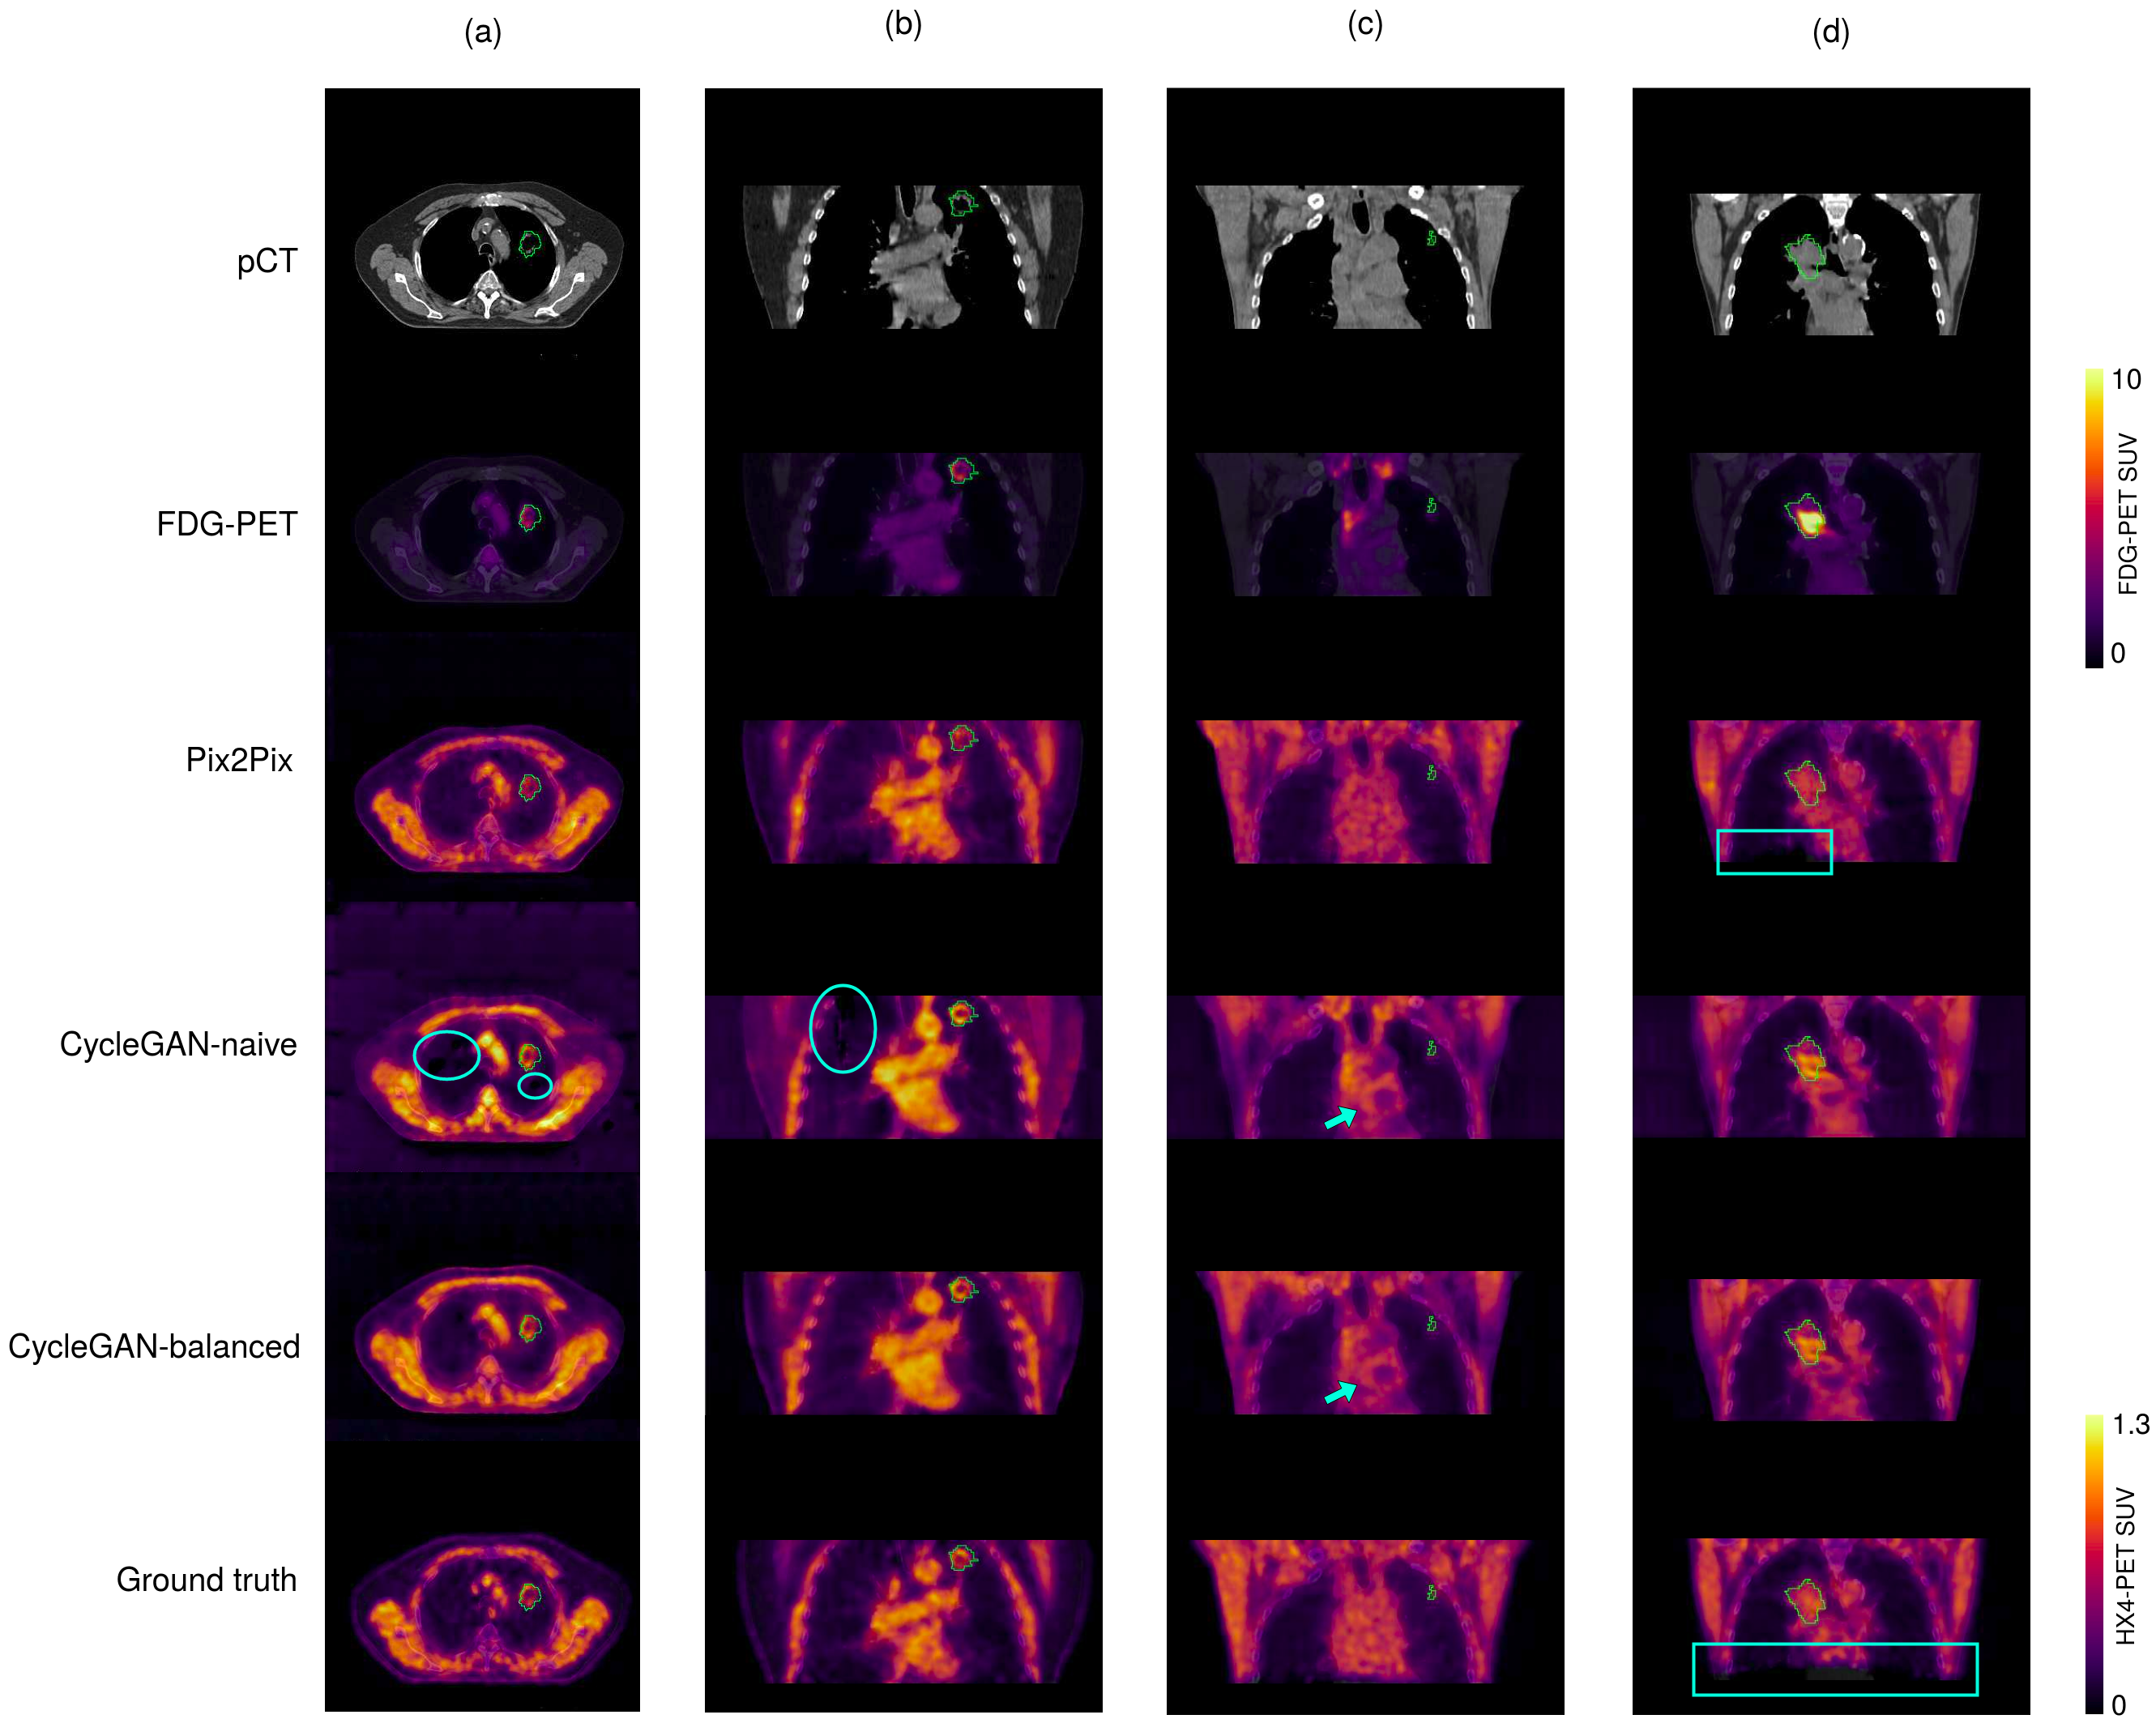
\includegraphics[width=1.4\linewidth]{figures/Expt_2/image_quality/image_quality_inspection_viz-2.png}
    }
    \caption{Corresponding slices of the inputs, the ground truth and the predictions. Gross tumor volumes (GTV) are delineated with green contours. Severe background noise is visible in CycleGAN-naive outputs, which also penetrates into the foreground as seen in (a). Sharp edged holes in (a) and a rift in (b) (cyan ellipses), a common occurrence in CycleGAN-naive predictions. In (d), the Pix2Pix output shows structure break at the bottom likely caused due to model being trained on faulty ground truth (cyan bounding boxes). In (c), the outputs of CycleGAN-naive and CycleGAN-balanced have a hallucinated ring-shaped hypoxia signature near the heart (cyan arrows).}
    \label{fig:hx4_image_quality_inspection_viz}
\end{figure}

None of Pix2Pix predictions contained severe background noise patterns, as opposed to the predicted images from CycleGAN-naive, all of which were severely corrupted by noise in both background and foreground. CycleGAN-balanced stands almost half-way between the other two models in terms of background and foreground noise, although none of its outputs contained noise as severe as in case of CycleGAN-naive. The background noise is easily visible in Figure \ref{fig:hx4_image_quality_inspection_viz}a. The presence of greater noise in CycleGAN-naive is likely to be related to its conceptual problem related to non-invertibility. The \textit{A}$\rightarrow$\textit{B} translation involves predicting hypoxia map from pCT and FDG-PET, which can have a unique solution. Whereas its reverse, the \textit{B}$\rightarrow$\textit{A} translation, involves computing ideally exact pCT and FDG-PET given only the hypoxia map information, which is not possible unless the model encodes the extra information, as noise or artifacts, in the hypoxia image.

Structural breaks and holes were observed in a majority of all models' outputs. These were, however, more severe and numerous in case of CycleGAN-naive and CycleGAN-balanced, more in the former than in the latter. Pix2Pix had comparably lower number of these faults. A notable difference is that while many of such structural faults appeared in roughly the middle and upper regions of the body in predicted images in case of the two CycleGANs, most of them in Pix2Pix predictions were located in the bottom-most axial slices. These are shown in Figures \ref{fig:hx4_image_quality_inspection_viz}a, \ref{fig:hx4_image_quality_inspection_viz}b and \ref{fig:hx4_image_quality_inspection_viz}d. A likely cause of this is the registration imperfections in the ground truth HX4-PET-reg images, many of which had missing signal in parts of the bottom axial slices. Pix2Pix training, which assumes voxel-to-voxel similarity across input and output images, might have been affected by this training noise resulting in a model that couldn't accurately predict the hypoxia patterns in the bottom slices. On the other hand, the CycleGAN models which were trained on unpaired and unregistered HX4-PET-unreg images did not exhibit structural breaks of this kind, and in fact, during validation, were able to predict plausible hypoxia patterns in the bottom slices of their predictions whose corresponding ground truths themselves were faulty. This is visible in Figure \ref{fig:hx4_image_quality_inspection_viz}d. The fact that the validation set's ground truth HX4-PET-reg images have this issue of missing signal may create another problem -- if the reference image itself is partly incomplete in some region and if a model predicts a plausible hypoxia signal in that region of its predicted image, evaluating the image quality, especially using the voxel-wise difference metrics, can result in an incorrect assessment. However, this may not pose a serious issue here because first, only a small portion of the signal in entire ground truth image is missing, and second, the models being compared have significant differences in performance as the visual inspection revealed.

Finally, the type of image degradation related to the presence of hallucinated structures was observed more commonly in case of CycleGAN-naive and CycleGAN-balanced as compared to Pix2Pix. This was mainly characterized by the insertion of ring-shaped hypoxia signatures in regions near the heart and the upper abdomen. However, such signatures are a common feature only within the tumor where parts of its periphery are actually hypoxic. A likely reason of this pattern to occur in other regions in the predictions of the two CycleGANs is the failure to learn relevant anatomical features from the pCT and depending more heavily on features related to metabolic activity from FDG-PET in these regions. The Pix2Pix model trained directly in a supervised manner mostly managed to avoid this issue. This can be seen in Figure \ref{fig:hx4_image_quality_inspection_viz}c.

In summary, the results of the visual inspection reflect the quantitative evaluation results. Pix2Pix produced synthetic HX4-PET images that are visually highly similar to the ground truth, mostly owing to its supervised training. However, because it was trained in the supervised manner on imperfect ground truth images, it also produced locally specific structure breaks in its predictions. Among the unpaired GAN systems, CycleGAN-balanced showed great improvement over CycleGAN-naive and was able to greatly reduce degradation caused by noise and hallucinated structures.


% ------------------------------------------------------------------------------
\subsection{Results and Analysis 2: Analyzing Model Convergence during Training}
\label{cycelgan_convergence}


\subsubsection{Adversarial training of CycleGAN} 
Informally, model convergence refers to a case where the machine learning model's loss approaches a certain optimal value with a decreasing rate over the training iterations. In GAN training, two networks are simultaneously optimized with conflicting objectives. In theory, a Vanilla GAN model asymptotically converges to an equilibrium state where the generator perfectly models the data distribution and the discriminator's prediction over real and fake data is 0.5 on average, i.e. it can only do random guessing \cite{goodfellow2014generative}. This stands, of course, only under the condition that the discriminator is trained to optimality for each iteration of the generator's update. In practice, the discriminator is updated just once per generator update, but since the discriminator's task of binary classification is simpler than the generator's task of image synthesis, the discriminator is likely to learn faster and remain competitive with the generator in the corresponding iterations. In this part of the experiment, GAN convergence is analyzed empirically for the CycleGAN-naive and CycleGAN-balanced systems, by reasoning based on their recorded training losses.

The least-squares adversarial loss used in our CycleGAN models is shown in Equation \ref{eq:gan_loss}.
\begin{equation}
    \begin{aligned}
    L(G) &= E_{x \sim p_{data}(x)} [(D(G(x)) - 1)^2] \\
    L(D) &= E_{y \sim p_{data}(y)} [(D(y) - 1)^2] + E_{x \sim p_{data}(x)} [D(G(x))^2]
    \end{aligned}
    \label{eq:gan_loss}
\end{equation}
where $G$ and $D$ represent a generator ($G_{AB}$ or $G_{BA}$) and the corresponding discriminator ($D_B$ or $D_A$), respectively. $x$ represents an image from the input domain of the generator $G$, and $y$ represents an image from its target domain. This general representation is used here for simplicity. 

During training, $G$ and $D$ are updated in an alternating manner. As the training progresses and if the training is stable, both $G$ and $D$ improve at a similar rate maintaining a competitive behavior. Depending on the extent of the stability, losses of both models either stay constant reaching an equilibrium or oscillate around the equilibrium values. Such an equilibrium state is reached when, after every update, $G$'s output images are good enough to force $D$ into random guessing and predicting a validity value of 0.5 on average for both real and fake images. Then according to Equation \ref{eq:gan_loss}, the equilibrium state loss values $L(G^*)$ and $L(D^*)$ are 0.25 and 0.5, respectively. 

\begin{figure}[h!]
    \begin{subfigure}{.5\textwidth}
        \centering
        \includegraphics[width=.95\linewidth]{figures/Expt_2/gan_convergence/loss_G_AB.png}
        \caption{}
        \label{fig:loss_G_AB}
    \end{subfigure}
    \begin{subfigure}{.5\textwidth}
        \centering
        \includegraphics[width=.95\linewidth]{figures/Expt_2/gan_convergence/loss_D_B.png}
        \caption{}
        \label{fig:loss_D_B}
    \end{subfigure}
    \newline

    \begin{subfigure}{.5\textwidth}
        \centering
        \includegraphics[width=.95\linewidth]{figures/Expt_2/gan_convergence/loss_G_BA.png}
        \caption{}
        \label{fig:loss_G_BA}
    \end{subfigure}
    \begin{subfigure}{.5\textwidth}
        \centering
        \includegraphics[width=.95\linewidth]{figures/Expt_2/gan_convergence/loss_D_A.png}
        \caption{}
        \label{fig:loss_D_A}
    \end{subfigure}
    
    \begin{subfigure}{.5\textwidth}
        \centering
        \includegraphics[width=.95\linewidth]{figures/Expt_2/gan_convergence/loss_cycle_A.png}
        \caption{}
        \label{fig:loss_cycle_A}
    \end{subfigure}
    \begin{subfigure}{.5\textwidth}
        \centering
        \includegraphics[width=.95\linewidth]{figures/Expt_2/gan_convergence/loss_cycle_B.png}
        \caption{}
        \label{fig:loss_cycle_B}
    \end{subfigure}

    \caption{Adversarial and cycle consistency loss curves for the two CycleGAN models. Exponential moving average smoothing was applied to each to show the general trend.}
    \label{fig:cyclegan_losses}
\end{figure}{}

Figure \ref{fig:cyclegan_losses} shows the adversarial training loss plots for CycleGAN-naive and CycleGAN-balanced. The aforementioned general reasoning is now applied independently to the two generator-discriminator pairs of the CycleGAN system. Consider the \textit{A}$\rightarrow$\textit{B} direction first. The adversarial loss $L({G_{AB})}$ of CycleGAN-balanced was closer to the equilibrium value than the that of CycleGAN-naive was, whose $G_{AB}$ was much more unstable and diverged away more significantly from around 25,000$^{th}$ iteration. This effect relates to the corresponding discriminator $D_B$ of CycleGAN-naive starting to overpower its $G_{AB}$ at around the same period. Discriminator $D_B$ of CycleGAN-balanced was maintained more stably around its equilibrium loss value of 0.5 over the full training period. Now looking at the \textit{B}$\rightarrow$\textit{A} direction, a similar pattern is observed. Except here, the generator-discriminator pair $G_{BA}$ and $D_A$ of CycleGAN-balanced appeared to destabilize and deviate away between 40,000$^{th}$ and 50,000$^{th}$ iteration, although eventually regaining stability near the end of the training. 

Additionally, cycle-consistency in CycleGAN-balanced was maintained to a greater extent almost throughout the training period as compared to CycleGAN-naive. The desirable training characteristics shown by the CycleGAN-balanced system can be attributed to its design modification.

\begin{figure}[h!]
    \makebox[\textwidth][c]
    {
        \begin{subfigure}{.4\textwidth}
            \centering
            \includegraphics[width=\linewidth]{figures/Expt_2/gan_convergence/metric_val_mse.png}
            \caption{}
            \label{fig:metric_val_mse}
        \end{subfigure}
        \begin{subfigure}{.4\textwidth}
            \centering
            \includegraphics[width=\linewidth]{figures/Expt_2/gan_convergence/metric_val_mae.png}
            \caption{}
            \label{fig:metric_val_mae}
        \end{subfigure}
        \begin{subfigure}{.4\textwidth}
            \centering
            \includegraphics[width=\linewidth]{figures/Expt_2/gan_convergence/metric_val_psnr.png}
            \caption{}
            \label{fig:metric_val_psnr}
        \end{subfigure}
    }
    \newline
    \makebox[\textwidth][c]
    {
        \begin{subfigure}{.4\textwidth}
            \centering
            \includegraphics[width=\linewidth]{figures/Expt_2/gan_convergence/metric_val_ssim.png}
            \caption{}
            \label{fig:metric_val_ssim}
        \end{subfigure}
        \begin{subfigure}{.4\textwidth}
            \centering
            \includegraphics[width=\linewidth]{figures/Expt_2/gan_convergence/metric_val_nmi.png}
            \caption{}
            \label{fig:metric_val_nmi}
        \end{subfigure}
        \begin{subfigure}{.4\textwidth}
            \centering
            \includegraphics[width=\linewidth]{figures/Expt_2/gan_convergence/metric_val_histogram_chi2.png}
            \caption{}
            \label{fig:metric_val_histogram_chi2}
        \end{subfigure}
    }
    \caption{Validation metrics for the two CycleGAN models over the training period.}
    \label{fig:cyclegan_metrics}
\end{figure}{}

\subsubsection{Generalization performance} 
Next, we examine whether the same trend as was observed in the training convergence parameters is reflected in the models' generalization performance on the validation set. Figure \ref{fig:cyclegan_metrics} plots the six validation metrics for the CycleGAN models over the training period. The voxel-wise difference metrics -- MSE, MAE and PSNR -- show a generally consistent improvement in CycleGAN-balanced reflecting its relatively stable training. However, the metrics based on image intensity statistics -- SSIM, NMI and histogram $\chi^2$ distance -- show a brief, yet prominent, performance dip in the model halfway into the training suggesting a temporary drop in its generalizability. CycleGAN-naive followed a generally similar trend as CycleGAN-balanced up until approximately 25,000$^{th}$ iteration -- i.e. gradual improvement in the beginning followed by a performance dip. Though, contrary to CycleGAN-balanced, it was unable to recover its generalizability and continued to worsen. This correlates with the significant instability and divergence of the CycleGAN-naive model observed in the training convergence parameters at about the same period in the training process.

In summary, the image quality metrics applied on validation data were indeed informative about model convergence. Additionally, since some of them measured different properties of the generated images, they can be helpful in effectively tracking model generalizability.



%%%%%%%%%%%%%%%%%%%%%%%%%%%%%%%%%%%%%%%%%%%%%%%%%%%%%%%%%%%%%%%%%%%%%%%%%%%%%%%%%%%%%%%%%%%%%%%%%%%%%%%%%%%%%%%%%%%%%%%%%%%%%%%%%%%%%%%%%%%%%%%
\section{Experiment 3: Application-specific Downstream Tasks}
\label{Expt_3}
This experiment focuses on clinical evaluation of the synthetic hypoxia PET images by quantifying hypoxia inside the gross tumor volume (GTV).


% ---------------------------
\subsection{Experiment Setup}
HX4-PET-syn images are computed for each patient in the validation set using the fully trained models, their units converted to SUV scale, and stored as NRRD files. The images are then loaded and analyzed. Each HX4-PET-syn image and its corresponding ground truth HX4-PET-reg are first cropped to a bounding box containing just the GTV. The GTV mask is then applied to the images, and intensities outside the mask are set to 0. Next, the GTV SUV values are converted to the tumor-to-background ratio (TBR) by dividing each GTV voxel's SUV with $SUV_{aorta-mean}$. From this point onward, the different hypoxia quantification metrics are computed separately as follows:

\begin{enumerate}
    
    \item \textit{MSE-GTV and SSIM-GTV:} MSE and SSIM are calculated only on the GTV voxels using array masking.
    
    \item \textit{Hypoxic tumor classification:} One of the ways of classifying the tumor as hypoxic or non-hypoxic is by calculating the total physical volume of the hypoxic region in the GTV, known as hypoxic volume (HV), and applying a threshold. We calculate HV by first performing point-wise intensity thresholding using standard TBR threshold of 1.4 (Zegers et al. \cite{zegers2013hypoxia}) to obtain a binary image of hypoxic voxels followed by calculating the total physical volume (in mm$^3$) occupied by them. Then, HV threshold of 1 cm$^3$ is applied beyond which the tumor is classified as hypoxic, similar to Even et al. \cite{even2017predicting}. Tumor classification is performed for each predicted image and its corresponding ground truth, and the mean accuracy is derived.
    
    \item \textit{Hypoxic region segmentation:} The 3D hypoxic region in the GTV is segmented by applying the standard TBR threshold of 1.4. This is performed for each predicted image and its corresponding ground truth image. Then, the Dice Similarity Coefficient (DSC) is used to measure the overlap between the hypoxic regions. 

\end{enumerate}


% -------------------------------
\subsection{Results and Analysis}
Table \ref{tab:hypoxia_metrics} reports the mean values of the hypoxia quantification measures over the validation set. The quantitative results provide no conclusive evidence on the model performances and are, in fact, slightly contradictory to previous results. MSE-GTV and SSIM-GTV were very similar for all the models, and Pix2Pix was less competent in accurately predicting the hypoxic regions. CycleGAN-balanced didn't show an improvement over CycleGAN-naive here. A visualization of the predicted tumor hypoxia patterns is shown in Figure \ref{fig:hypoxia_viz}. Two important observations can be made are. First, the Pix2Pix outputs show significant checkerboard-like noise patterns. Note that these are of different nature compared the image-wide foreground noise defined as a failure criterion earlier in experiment \ref{Expt_2} in that these are of higher frequency and are localized to high-intensity regions, such as the tumor locality shown in the figure. Predictions from the CycleGANs show minimal noise. Second, Pix2Pix predictions do not contain sufficiently high intensity regions to be capable of being segmented and their spatial patterns do not match the hypoxic patterns in the ground truth. Since only a small number of voxels carry sufficiently high intensity values, there existed many false-negative voxels which collectively amounted to hypoxic tumors being misclassified as non-hypoxic. In case of the CycleGANs, their predicted hypoxic patterns are more similar to the metabolic patterns from FDG-PET, instead of the ground truth.

\begin{table}[h!]
    \footnotesize
    \centering
    \makebox[\textwidth][c]
    {
        \begin{tabular}{ccccc}
            \textbf{Method}   & \textbf{MSE-GTV}   & \textbf{SSIM-GTV}   & \textbf{Tumor classif. accu.}   & \textbf{Hypoxic region seg. Dice} \\
            \hline
            Pix2Pix   & \textbf{0.067} $\pm$ 0.040   & 0.870 $\pm$ 0.082   & 61.2\% (12/19)   & 0.058 $\pm$ 0.092 \\
            CycleGAN-naive   & 0.079 $\pm$ 0.046   & \textit{0.884} $\pm$ 0.066   & \textbf{78.9}\% (15/19)   & \textbf{0.141} $\pm$ 0.184 \\
            CycleGAN-balanced   & \textit{0.068} $\pm$ 0.042   & \textbf{0.886} $\pm$ 0.066   & \textit{73.7\%} (14/19)   & \textit{0.127} $\pm$ 0.174 \\
        \end{tabular}
    }
    \caption{Results of tumor hypoxia quantification. Best and second-to-best values are highlighted with bold and italics font, respectively. For tumor classification, the accuracy is given in percentage values and fraction of patients with correctly classified tumors.}
    \label{tab:hypoxia_metrics}
\end{table}

\begin{figure}[h!]
    \centering
    \makebox[\textwidth][c]
    {
        \includegraphics[width=1.1\linewidth]{figures/Expt_3/hypoxia_viz.png}
    }
    \caption{Tumor hypoxia patterns generated by the models. GTV is delineated with green contour, and the hypoxic region in each of three models' prediction and the ground truth is marked with blue contours. In both examples, Pix2Pix predictions didn't contain sufficiently intense regions, hence no hypoxic areas are seen segmented in these slices.}
    \label{fig:hypoxia_viz}
\end{figure}

One of the reasons Pix2Pix fails here appears to be related to its supervised training. The ground truth images contain registration errors that are more pronounced at the small scale in which this evaluation is performed. The fine hypoxia patterns in the ground truth, including those within the tumor, might have shifted post-registration causing misalignment with the CT and FDG-PET features, thereby inducing noise in the paired training data. Therefore, although the Pix2Pix model could produce synthetic hypoxia images of an overall higher quality, these images reveal large inaccuracies when examined at the scale of the tumor.
In case of the two CycleGANs, the tumor hypoxia patterns matched the spatial pattern of FDG uptake suggesting that the models learned to excessively depend on FDG-PET features. Another reason for poor clinical performance of all three models might be the small size of the training dataset. Even when using a patch-based training approach, the number of sufficiently varied training samples was very low. Training on a larger dataset could likely improve performance.

\chapter{Discussion}
\label{Discussion}

% Research qs were answered
Through experiments \ref{Expt_1} and \ref{Expt_2}, we show that the paired Pix2Pix approach can generate higher quality images as compared to unpaired CycleGAN, although at the cost of acquiring and preparing the ground truth images. Among the two CycleGAN systems, CycleGAN-balanced was able to circumvent the non-invertibility issue of CycleGAN-naive due to its design modification, and produced better results as indicated by both quantitative and qualitative analyses. Our quantitative evaluation of the synthetic HX4-PET images involved using a set of six full-reference metrics that measured broadly two different aspects of the images -- voxel-wise accuracy and (local and global) image statistics. Furthermore, each metric has its own unique property and since the ``quality" of an image is multifaceted in nature, using a population of such metrics for image assessment can more effectively capture image quality as compared to using a smaller subset of them. We thereby address our first research question. In \ref{cycelgan_convergence}, we perform an analysis of CycleGAN training losses over the training period and observe that the CycleGAN-balanced model was more stable and displayed better convergence properties as opposed to the CycleGAN-naive model which diverged away from its objectives. The validation metrics collectively reflected up to a great extent the similar trends as the convergence parameters, thereby providing an answer to our third research question. Finally, through experiment \ref{Expt_3}, we address our second research question by identifying and performing clinically useful downstream tasks to determine the value of our synthetic HX4-PET images. Tumor hypoxia measurement as derived from synthetic images predicted by Pix2Pix showed poor 
As supplementary material, we supply the \textit{WandB} training reports for the depth-estimation task (experiment \ref{Expt_1}) \footnote{Training report for the depth-estimation task: \url{https://bit.ly/3x452Qi}} and for the HX4-PET synthesis task (experiment \ref{Expt_2}) \footnote{Training report for the HX4-PET synthesis task: \url{https://bit.ly/35Y8dx2}} which include training losses, validation metrics and intermediate outputs of the models.

% Some limitations, and opportunities for future work (stuff to do after thesis):
%   1. Dataset size -- larger training set to train better models, larger validation set to test properly
%   2. CycleGANs appeared to focus more on FDG features. Would be nice to see through an ablation study whether or not they really use CT features. One way to do this is taking the same trained models, turning off the CT signal in their input and performing inference.
%   3. With metrics - Need to consult more theoretical literature to understand their mathematical properties. This would allow choosing better and more diverse metrics to use and evaluate with the voting method.
%   4. Turing test
There are several limitations of this thesis which can provide opportunities for future work. First, the small size of our Maastro Lung HX4-PET dataset was a serious limitation on model training and validation. A larger training dataset would allow training better translation models, and a sufficiently large and diverse validation dataset would enable more effective evaluation of the models. Second, it was observed that both the CycleGAN models predicted tumor hypoxia patterns which closely resembled the FDG uptake signatures rather than the actual spatial distribution of hypoxia. The models might have learned to heavily rely on FDG-PET features, while ignoring CT information. It would be interesting to verify this by performing an ablation study on these models. This could be conducted, for instance, by performing inference on the fully trained models with the CT signal set to zero value and observing the generator outputs. Third, the quality assessment of the synthetic HX4-PET images was performed using a set of six general-purpose image quality and similarity metrics that were logically chosen. However, this portfolio of evaluation metrics can be improved. It would be valuable to consult theoretical literature on image metrics and understand in a greater depth their mathematical properties. This would help in selecting more suitable and diverse metrics thereby improving the effectiveness of the consensus-based image evaluation. Fourth, as an extension of the simple automated clinical evaluation performed in experiment \ref{Expt_3}, a version of the Turing test can be performed by presenting the synthetic HX4-PET images to a radiation oncologist, with a certain clinically relevant goal, for instance, performing a prognosis based on the synthetic images and comparing with the prognosis done based on the ground truth.


% Fine tuning stuff (questionable. don't include)
% Second, the Pix2Pix model failed in accurately predicting tumor hypoxia and produced high-frequency noise patterns in the tumor region, although its synthetic HX4-PET images were of an overall high quality. In addition to the registration-related issues, this failure can also be attributed to model training. In addition to using a larger training dataset as a possible solution to reducing these artifacts, it would be interesting to investigate into \textit{fine tuning} the trained Pix2Pix model using the existing dataset. This could be performed, for instance, by first using a patch-sampling strategy that focuses more on the tumor vicinity. Then, the weights of the Pix2Pix generator's encoder (which is its feature extractor) could be frozen while updating only its decoder (which is its image synthesizer). The intuition behind this is that, in doing so, the noise patterns can potentially be reduced since they caused during the upsampling operations used the decoder path, and that this by learning better upsampling kernels


% Expt 3 stuff (need this? probably not)
% We argue that although none of our models' synthetic HX4-PET was clinically satisfactory, paired translation approaches such as Pix2Pix that assume voxel-wise alignment are bound to produce inaccuracies in their images at a scale of the tumor.
% In our dataset, HX4-PET scans for all patient were acquired on a different day from FDG-PET and pCT acquisition. A problem with tumor hypoxia is the fact that the hypoxic region has a tendency to change over time, even over a period of hours [cite ...]. Zegers et al. \cite{zegers2013hypoxia} raise this argument to explain the relatively low \textit{voxel-level} correlation they observed between FDG-PET and HX4-PET SUV values despite a significant correlation on \textit{tumor-level} properties between the two modalities. It is possible that in our data, the state of the tumor captured by FDG-PET/pCT might not correspond perfectly to its state captured by HX4-PET. In such a case, even if the HX4-PET image were to be perfectly registered over pCT and FDG-PET, a supervised method that assumes voxel-level correspondence would be less effective, to say the least. In this view, it could then be possible that the hypoxia patterns predicted by the CycleGANs, although not matching the ground truth, might reflect the ``actual" hypoxia distribution.
\chapter{Conclusion}
\label{Conclusion}

In this work, we posed the problem of predicting hypoxia from FDG-PET and CT scans as image-to-image translation, and investigated image translation GANs for synthesizing full HX4-PET images from the multimodal input. Using the paired Pix2Pix and the unpaired CycleGAN, we observed that the paired approach produces superior quality images both in our simulated translation task and in the HX4-PET synthesis task. We argue that the naive application of CycleGAN to the HX4-PET synthesis task has a conceptual flaw related to non-invertibility, and propose an alternative strategy to circumvent this problem while still requiring only unpaired training data. This modified CycleGAN system showed substantial performance improvement over the default CycleGAN in terms of image quality. To assess the quality of the synthetic HX4-PET images in a comprehensive manner, we construct a set of six measures of image quality and image similarity, of which three metrics -- MSE, MAE and PSNR -- measure the voxel-level accuracy of the the synthetic images with respect to the ground truth, whereas the remaining three -- SSIM, NMI and histogram distance -- account for the fidelity of image structure and statistics. A systematic visual inspection of the synthetic HX4-PET images validated the assessment of these metrics and also revealed common failure modes for each model. The Pix2Pix-generated images contained, on average, the least amount of degradation and artifacts, although they suffered from structural breaks in specific areas. These faults can be attributed to the supervised training of the Pix2Pix model which used ground truth images containing registration imperfections. Despite the clear performance difference across the three GAN models based on image quality, the clinical evaluation of their synthetic images conducted via tumor hypoxia quantification tasks produced mixed and inconclusive results. The Pix2Pix model performed remarkably worse in comparison with the two CycleGANs. While a majority of the tumors in the synthetic images produced by the CycleGAN models were classified correctly, the classification rate in Pix2Pix predictions is lower. However, as indicated by a poor segmentation score, none of the models could predict accurately the spatial distribution of high hypoxia. The primary reason could be the lack of sufficient training data, and the second reason, specifically for Pix2Pix, could be the noise in its supervision signal caused due to imperfect ground truth images. Given sufficient training data, unpaired models like CycleGAN, especially the modified version of it, could be more suitable for the HX4-PET synthesis task.

\bibliographystyle{unsrt}
\bibliography{Bibliography}
\end{document}
